%%%% ijcai20.tex

\typeout{IJCAI--PRICAI--20 Instructions for Authors}

% These are the instructions for authors for IJCAI-20.

\documentclass{article}
\pdfpagewidth=8.5in
\pdfpageheight=11in
% The file ijcai20.sty is NOT the same than previous years'
\usepackage{ijcai20}

% Use the postscript times font!
\usepackage{times}
\usepackage{soul}
\usepackage{url}
\usepackage[hidelinks]{hyperref}
\usepackage[utf8]{inputenc}
\usepackage[small]{caption}
\usepackage{graphicx}
\usepackage{subfig}
\urlstyle{same} % DO NOT CHANGE THIS

\usepackage{amsmath}
\usepackage{amsthm}
\usepackage{booktabs}
\usepackage{algorithm}
\usepackage{algorithmic}
\urlstyle{same}
\usepackage{amsmath,amssymb,amsfonts}
\usepackage{algorithmic}
\usepackage{textcomp}
\usepackage{xcolor}
\usepackage{multirow}
\usepackage{todonotes}
\usepackage{soul}


\newcommand{\context}{c}
\newcommand{\expect}{\mathbb{E}}
\newcommand{\expectdiff}{ED}
\newcommand{\scorediff}{SD}
\newcommand{\latentvariables}{\mathbf{z}}
\newcommand{\inference}{q}
\newcommand{\generation}{p}
\newcommand{\hiddenstate}{\mathbf{h}}
\newcommand{\state}{\mathbf{s}}
\newcommand{\action}{\mathbf{a}}
\newcommand{\reward}{r}
\newcommand{\goal}{g}
\newcommand{\player}{pl}
\newcommand{\pindex}{i}
\newcommand{\prior}{p}
\newcommand{\bin}{\beta}
\newcommand{\boxscore}{b}
\newcommand{\home}{\it{Home}}
\newcommand{\away}{\it{Away}}
\newcommand{\none}{\it{Neither}}
\newcommand{\team}{\it{team}}
\newcommand{\egoal}{\it{goal}}
\newcommand{\Qobs}[2]{Q_{#1}^{\it{obs}}(#2)}
\newcommand{\Qmodel}[3]{\hat{Q}_{#1}(#2,#3)}
\newcommand{\Qbin}[2]{\hat{Q}_{#1}(#2)}
\newcommand{\features}{\boldsymbol{x}}
\newcommand{\softmax}{\boldsymbol{\phi}}
\newcommand{\sigmoid}{\boldsymbol{\sigma}}
\newcommand{\observation}{\boldsymbol{o}}
\newcommand{\GaussianParameters}{\boldsymbol{\omega}}
\newcommand{\BernoulliParameters}{\theta}

\newcommand{\oliver}[1]{\textcolor{red}{Oliver: #1}}



\title{Learning Deep Hockey Player Representations with \\ A Variational Hierarchical Encoder}
% \title{Learning Deep Contextualized Representations for Hockey Players}
%\title{Deep Contextualized Player Representations}

% \title{Deep Contextualized Player Representations with \\ A Variational Hierarchical Encoder}
\author{Anonymous Authors\\(Do Not Distribute)}

\begin{document}
\maketitle


\begin{abstract} Computing the expected impact of player actions is one of the key problems in sports analytics. To capture a player's influence on action outcomes, we learn {\em contextualized representations for hockey players} using a new model: Variational Hierarchical Encoder with Recurrence (VHER). VHER conditions on the match context (current observation and game history) to predict the acting player (e.g., the player possessing the puck). We apply variational inference to learn a context-specific shared prior, which induces a shrinkage effect for the posterior player representations. The player representations are validated in downstream sports analytics tasks.  Experimental results show the state-of-the-art performance of VHER in the tasks of (1) identifying the acting player, (2) estimating expected goals, and (3) predicting the final score differences.
\end{abstract}


% \iffalse 
% things to do for ijcai
% \begin{enumerate}
    
%     \item try deterministic player representation using Gaussian parameters for the posterior. Trying different methods: mean, mean-variance, random sample. check
%     \item check for references on using code as embeddings, maybe check vision papers. couldn't find any.
%     \item I wonder if this would finally work to predict the team that is playing. Tried and failed.
%     \item baselines: how about generic auto-encoder type setup with RNN applied to one-hot vectors? So the input is a one-hot vector and the output is a categorical distribution? Or is that what you mean by "deterministic embedding"? Deterministic function from (state, action) to playerid. tried baselines.
%     \item experiments: actually I don't know exactly how the player identification results are computed. E.g. for the VAE testing of $P(pl_t)$ do you sample from the posterior $q(z|pl_t)$? Answer: we add the prior representation as input to the LSTM. Cite Bengio? I don't quite understand the DE either. cgecj
% \end{enumerate}
% \fi

\section{Introduction}
% action value evaluation -> generating player representation ->limitation of word2vec kinds embedding model -> contextual embedding -> latent variable embedding. 
% With the advancement of high-frequency optical tracking and object detection systems, m
More and larger event stream datasets for sports matches 
%have increased the opportunities  for applying 
% require 
facilitate applying advanced 
machine learning to model complex sports dynamics.
Many recent works~\cite{Liu2018,decroos2018action,fernandez2019decomposing} have proposed to estimating the team success following a player's actions. These estimated action values support many downstream applications, such as game outcomes predictions or player evaluation. However, when estimating action impact, previous works often 
% overlook the player-specific features (e.g. scoring ability) 
assign the same values to actions performed by different players. Neglecting differences among individual players compromises the model performance. 

% \todo[inline]{to Pascal and Mike: do you think it takes too many words to introduce the background before we move to our work?\\Mike: No, your coverage of previous work ends and your description of your own contribution begins roughly where I would expect it to.} 
The most common approach to incorporating player information in sports statistics is to use a {\em hierarchical model} \cite{kruschke2014doing,Gelman06}. Existing hierarchical models in sports assume a fixed parametric form (e.g. linear or categorical), and learn different parameter estimates for each player. In a Bayesian hierarchical model, the posterior parameter distribution for each player is shrunk toward the mode of a shared prior. {\em Shrinkage} substantially reduces the estimation of variance~\cite{Murphybook12}, but it is hard to find a suitable distributional form for the complex dynamics of team sports.

Neural networks are general function approximators well-suited to capturing sports dynamics.
% The most straightforward uses a one-hot vector representation of player identity (pid) and trains a neural net to dynamically learn the correlations between pids and game context~\cite{Le2017}.
% given its ability of modeling non-linear relation between input features.
% Despite of simplicity, there is no guarantee the neural network will always recognize this relation without explicitly modeling the player information. 
% The one-hot representation is not informative enough for a neural network to adequately model the connection between individuals and team success, as our experiments below show.
% As evidence, our experiment shows very limited improvement when we directly complement the input space with pids.
%To achieve a more informative representation,
A recent work~\cite{ganguly2018problem} built a neural encoder to embed players.
% \st{They extracted the middle layer from the trained encoder and used it as a player embedding to facilitate the training of other primary tasks.}
They trained the encoder as a deterministic regressor, mapping game contexts to the identity of present players.
Their model, however,  shows large estimation variance, especially when the player presence has a multimodal distribution.

\begin{figure}[t!]
    \centering
    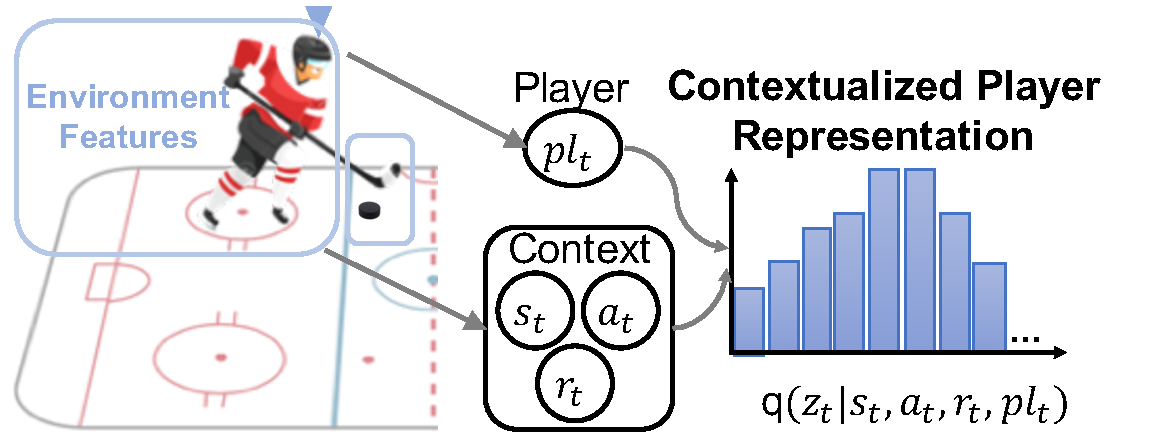
\includegraphics[width=0.4\textwidth] 
    {./figures/player-embedding-example.eps}
    \caption{The contextualized player representation, where we sample embeddings (latent variables) $\latentvariables_{t}$ for player $\player_{t}$ under game context ($\state_{t},\action_{t}$). $\state_{t}$ contains game history information (see section~\ref{sec:context-nhl}).
    } 
    \label{fig:player-represent}
\end{figure}

% A strength of Variational Auto-Encoders (VAE) is that they produce a distribution over outcomes that accommodates multiple modes. 
% % Without modeling the uncertainty, their deterministic embedding model generates large training variance and achieves only limited performance.


To leverage the advantages of both hierarchical models and neural approximators, we introduce a new model for learning player representations: the Variational Hierarchical Encoder with Recurrence (VHER). VHER is a neural hierarchical model.  Variational inference is applied to represent the player information in latent variables under different game contexts (current observations and game history, see Figure~\ref{fig:player-represent}).
% VHER formalizes the intuition that {\em similar players appear in similar contexts}.

The {\it neural hierarchical model} is based on the following generative process. 1) Sampling a vector of latent variables from a context-specific prior. The prior incorporates the information of both current observation and game history (with a LSTM), which forms a reliable representation of game context. 2) Using the latent variables to compute 
% the following generative process. Sample a vector of latent variables from a context-specific prior. 2) Compute 
categorical parameters that predict the currently acting player. The entire process can be interpreted as a predictive model that identifies the acting player given a game context.

During {\it variational inference}, we compute the approximate posterior for player representation conditioning on the current game context.
To determine the variational training objective, an Evidence Lower Bound (ELBo) is derived to be our loss function. 
The ELBo loss has two desirable properties. 1) It encourages the posterior representation for each player to shrink toward the mode of the context-specific prior. It naturally formalizes the intuition that {\em similar players appear in similar contexts}. 2) It reconstructs the acting player using a {\em multimodal} posterior player representation which guarantees the representation can accurately match the target player. 
% It guarantees the diversity of the posterior player representations where we can sample the continuous-value player embedding vectors.
% Both the shrinkage effect and embedding diversity are well present in an Evidence Lower Bound (ELBo).

% To demonstrate the effectiveness of our embedding model, w
We evaluate the predictive performance of our hierarchical model for identifying acting players, and evaluate the player representations in two external application tasks: predicting expected goals and final score difference (Figure~\ref{fig:flow-chart} concludes the entire process). Experimental results show the improvement of our VHER model over several comparison methods.
% \textcolor{blue}{shall we abandon the terminologies of 'secondary or primary task', it seems those terminologies won't help.}

\paragraph{Contributions.} The main contributions of this paper are:

\begin{itemize}
 \item A novel neural hierarchical model for learning representations of both players and game contexts. The model can be applied to learn representations for dynamic individual behaviour in domains other than sports. 
 \item A variational ELBo loss for representation learning that shares statistical strength among the observations of different agents through a shrinkage effect.
 \item To our best knowledge, the first {\em contextualized} player representations for professional sports.
\end{itemize}


\section{Related Works}
In this section, we describe the most related previous works.
\paragraph{Variational Auto-Encoder (VAE).} VAE has achieved promising performance in recovering multimodal distributions and in generating many kinds of complicated data, including handwriting~\cite{kingma2013auto}, image trajectories~\cite{WalkerDGH16} and player actions~\cite{mehrasa2019variational}.
VAEs apply a set of latent variables $\latentvariables$ to capture the variations of observed variables $\observation$.
During the generative process, the prior distribution of $\latentvariables$ is generally chosen to be a standard Gaussian $\mathcal{N}(0,1)$.
VAEs model the likelihood function $\generation(\observation|\latentvariables)$ with a neural {\it decoder} that applies a highly non-linear mapping from $\latentvariables$ to $\observation$.
% The non-linearity in $\generation(\observation|\latentvariables)$ leads to the intractable inference of 
As the true posterior $p(\latentvariables|\observation)$ is intractable, VAE approximates the true posterior with a {\it encoder}  $\inference(\latentvariables|\observation)$. The encoder models the approximate posterior distribution of $\latentvariables$ with a Gaussian: $\latentvariables\sim\mathcal{N}[\boldsymbol{\mu}, diag(\boldsymbol{\sigma}^{2})]$ ($\boldsymbol{\mu}$ and $\boldsymbol{\sigma}$ are computed as functions of observations $\observation$).
Parameters of the decoder and encoder are optimized to maximize a lower bound of the marginal likelihood of observations $p(\observation)$:
\vspace{-0.1in}
\begin{align}
    % & \log p(x) \geq \mathcal{L}(p(\observation))\\
     \hspace{-0.1in}\mathcal{L}(p(\observation))&=-KLD(\inference(\latentvariables|\observation)||p(\latentvariables))+\mathbb{E}_{\inference(\latentvariables|\observation)}\Big[\log\generation(\observation|\latentvariables)\Big]
\end{align}
\vspace{-0.15in}
% \todo{discuss neurips 2019 paper on hierarchical VAE}
% OS: I don't think we need this section. To make the estimations of $\expect[\inference(\latentvariables|\observation)]$ differentiable, ~\citeauthor{kingma2013auto} introduced an reparameterizing trick to sample from $\inference(\latentvariables|\observation)$ by:
% % \todo[inline]{What does $\player$ stand for?} 
% \begin{equation}
%     \mathbb{E}\Big[\log(\generation(\observation|\latentvariables))\Big]=\mathbb{E}\Big[\log \generation(\observation|\latentvariables=\boldsymbol{\mu}+\boldsymbol{\sigma}\odot\boldsymbol{\epsilon})\Big]
% \end{equation}
% where $\boldsymbol{\epsilon}\sim\mathcal{N}(0,1)$.

An extension~\cite{WalkerDGH16} designed a Conditional VAE (CVAE) that conditions the generation process on some external environment variables, but unlike our hierarchical model that computes the prior parameters, their conditional prior applies a standard Gaussian ($\mathcal{N}(0,1)$) during the generation process~\cite{Doersch16}.
The Variational Recurrent Neural Network (VRNN)~\cite{ChungKDGCB15} is an extension for sequential data, that combines VAE with LSTM recurrence. Variational inference is applied at every time step, but without conditioning on context variables, it does not provide contextualized representations. A recent work~\cite{KlushynCKCS19vae} proposed to learning a hierarchical prior for VAE, but their method focuses on only static images without considering the temporal dependency between continuous events.
% The object function is a timestep-wise variational lower bound:
% \begin{align}
%     %  \mathcal{L}\Big[\sum_{t=1}^{T}p(x_{t})\Big] = &
%      \sum_{t=1}^{T}\Big[-KL(\inference(\latentvariables_{t}|\observation_{\leq t},\latentvariables_{<t})||p(\latentvariables_{t}|\observation_{< t},\latentvariables_{<t}))+
%     & \log\generation(\observation_{t}|\latentvariables_{\leq t},\observation_{<t})\Big]
% \end{align}

\paragraph{Hierarchical Models in Sports Analytics.}
Many previous works~\cite{Gelman06,davis2015simulator}
% on shrinkage models 
have built multi-level hierarchical models for capturing player information in sports analytics and estimated the parameters of the posterior with Bayesian inference.
% Bayesian inference naturally incorporates the shrinkage effect into estimating model parameters. 
% % The shrinkage effect pulls the estimates of low-level parameters closer together than they would be if there was not a higher-level distribution, and generally, 
% The shrinkage effect encourages lower-level parameters to shift toward the mode of the higher-level distributions, which can significantly reduce the variance of estimation. 
% Similar hierarchical models have many applications in sports analytics, 
For example, ~\citeauthor{kruschke2014doing}(~\citeyear{kruschke2014doing}) built a hierarchical model to estimate the batting abilities for individual baseball players.
For each batter, they estimate the posterior probability of hitting the ball, from a prior conditioning on player positions.
Accordingly, for players in the same position, despite the difference in performance, their representations shrink toward the position-specific mode. 
% leaves the posterior distribution of their difference being nearly zero.
% Such a shrinkage effect can facilitate our player embedding model. Given the intuition that similar players are likely to appear in similar contexts, 
Our model achieves a similar shrinkage effect that encourages the posterior of player representation to shift toward the mode of a dynamic context-specific prior. A key difference is that neural networks can approximate general functions, whereas previous work on sports analytics assumed a known fixed functional or distributional form for the hierarchical model.

\paragraph{Contextualized Embedding.}
As a promising technique of incorporating background knowledge into representation learning, contextualized embedding has been extensively studied in Natural Language Processing (NLP). For example, ~\citeauthor{AkbikBV18}(~\citeyear{AkbikBV18}) proposed a contextual string embedding. The embedding model contextualizes words by their surrounding text. Therefore the same word will have different embeddings in different contexts. 
A recent work~\cite{PetersNIGCLZ18} used contextualized embeddings to model complex characteristics of word use (e.g., syntax and semantics).
%, and extended the application of embeddings across different linguistic contexts. 
They showed that contextualized embeddings can be easily added to existing models and significantly improved the state-of-the-art across six challenging NLP problems. The above embedding models are only applicable under the NLP environment where context and embedding targets are both words. In this work, we extend contextualized embeddings to the environment of professional sports and learn the player representations conditioning on complex game contexts.
% , we compute contextualized embeddings for NHL players conditioning on the game contexts (including the current observation and play history). 
% Our results also demonstrate the benefit of applying contextualized embeddings in identifying pids and predicting expected goals. 
% \textcolor{blue}{explain why we don't we compare with the word embedding model.}

\begin{figure}[t]
    \centering
    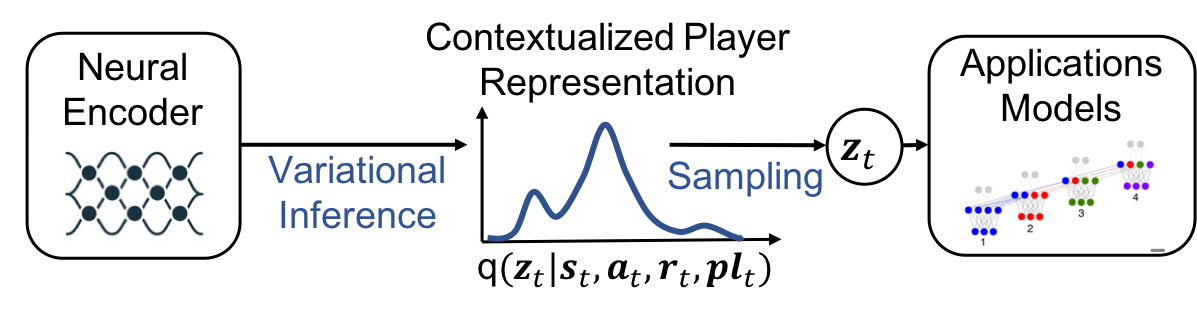
\includegraphics[width=0.5\textwidth] 
    {./figures/flow-chart.eps}
    \caption{System flow for learning contextualized player representations and validating them in the downstream application tasks.
    } 
    \label{fig:flow-chart}
\end{figure}

% \subsection{Agent Representations in RL?} 


% \section{Problem Formulation}
% \textcolor{blue}{Shorten the idea and place it under the introduction.}
% To utilize the player information, we formulate this task into two sub-problems: 1) How to learn a robust player embedding model and 2) How will the embedding influence the mode performance in solving the practical problem.

% For the first problem, we investigate the game environment, actions and games statistic that feature a player's overall playing skill.  
% To include the feature information into our embedding, our model is train to solve a secondary prediction problem: Given the condition a on-the-ball action $\action_{t}$, game context $\state_{t}$ (including locations, game time etc.) and play history $\hiddenstate_{t-1}$, who is likely to be the player   $\player_{t}$ performing the action. In this sense, our model summarizes all the conditional feature information into a embedding vector, and unlike previous works which assigns a deterministic embedding vector to each player, our model learns to generate a comprehensive embedding vector $\latentvariables_{t}$ conditioning on various game or player features. 

% To answer the second question, we look into two commonly studied problems including 1) game outcome prediction and 2) player performance evaluation. 
% In the recent years, many works have applied machine learning models to solve those problems, but a common drawback of the proposed models is they considered very limited player information.
% To overcome the limitation and validate our conditional embedding,
% % demonstrate the benefit of adding more player information
% , we input the learned player embedding vectors into their model and check whether and how the embedding will improve the model performances. 


\section{Play Dynamics in Ice Hockey}
This section introduces our NHL dataset and the approach to modeling play dynamics with contextual variables.
\subsection{Dataset}
We utilize a dataset constructed by NAME (name withheld to preserve anonymity).
% including player tracking and activity recognition. 
% It consists of play-by-play information of game events and player actions for the entire 2015-2016 NHL season. 
The data provides information about \textbf{game events} and \textbf{player actions} for the entire 2018-2019 NHL (largest professional ice hockey league) season,
which contains over 4 million events, covering 31 teams, 1,196 games and 1,003 players. 
% Table \ref{table:example-of-dataset} shows an excerpt. 
% A breakdown of this dataset is shown in table \ref{table:size-of-dataset}. 
% \begin{table}[htbp]
% \caption{Dataset Statistics.}
% \label{table:size-of-dataset}
% \begin{center}
% \begin{tabular}{|l|c|}
% \hline
% \bf{Number of Teams} & xx \\ \hline
% \bf{Number of Players} & x,xxx \\ \hline
% \bf{Number of Games} & x,xxx \\ \hline
% \bf{Number of Events} & x,xxx,xxx \\ \hline
% \end{tabular}
% \end{center}
% \end{table}
The dataset consists of events around the puck, and includes the identity and action of the player possessing the puck, with time stamps and features of the game context. 
We augment the data with derived features and list the complete feature set in Table \ref{table:feature-of-dataset}.
The table utilizes adjusted spatial coordinates where negative numbers denote the defensive zone of the acting player and positive numbers denote his offensive zone. Adjusted X-coordinates run from -100 to +100, Y-coordinates from 42.5 to -42.5, where the origin is at the ice center. The dataset records which unique player possesses the puck. {\em In the remainder of this paper, we refer to the acting player as the on-puck player.}
% As the dataset records only which player possesses the puck (= on-puck player), the term {\em ``acting player" refers to the on-puck player}.  but 
Our representation learning model can be extended to multiple players acting simultaneously given suitable multi-agent data.
%when given a dataset having the full observability of all players.

% \begin{table}[htb]
% % \caption{Complete Feature List}
% % \label{table:feature-of-dataset}
% \begin{center}
% \resizebox{\columnwidth}{!}{
% \begin{tabular}{|c|c|c|}
% \hline
% \bf{Name} & \bf{Type} & \bf{Range} \\ \hline
% X Coordinate of Puck & Continuous & [-100, 100]\\
% Y Coordinate of Puck & Continuous & [-42.5, 42.5]\\
% Velocity of Puck & Continuous & (-inf, +inf)\\
% Game Time Remain & Continuous & [0, 3600]\\
% Score Differential & Discrete & (-inf, +inf)\\
% Manpower Situation & Discrete & \{EV, SH, PP\}\\
% Event Duration & Continuous & [0, +inf) \\
% Action Outcome & Discrete & \{successful, failure\}\\
% Angle between puck and goal & Continuous & [$-3.14$, $3.14$]\\
% Home or Away Team & Discrete & \{Home, Away\} \\ \hline
% \end{tabular}
% }
% \end{center}
% \caption{Complete Feature List}
% \label{table:feature-of-dataset}
% \end{table} 

\begin{table}[]
\begin{tabular}{c|c|c}
\hline
Type & Name & Range \\ \hline\hline
\multirow{5}{*}{\begin{tabular}[c]{@{}c@{}}Spatial \\ Features\end{tabular}} & X Coordinate of Puck & {[}-100, 100{]} \\
 & Y Coordinate of Puck & {[}-42.5, 42.5{]} \\
 & Velocity of Puck & $(-\infty,+\infty)$ \\
 & Angle between & \multirow{2}{*}{\begin{tabular}[c]{@{}c@{}}[$-3.14$, $3.14$] \end{tabular}}\\ 
 & the puck and the goal & \\
 \hline
\multirow{2}{*}{\begin{tabular}[c]{@{}c@{}}Temporal \\ Features\end{tabular}} & Game Time Left & {[}0, 3,600{]} \\
 & Event Duration & (0, $+\infty$) \\ \hline
\multirow{4}{*}{\begin{tabular}[c]{@{}c@{}} In-Game \\ Features\end{tabular}} & Score Differential & $(-\infty,+\infty)$ \\
 & Manpower Situation & \{ES, SH, PP\} \\
 & Home or Away Team & \{Home, Away\} \\
% \multirow{2}{*}{\begin{tabular}[c]{@{}c@{}}Action\\ Type\end{tabular}} & Action Name & One-hot-vector \\
 & Action Outcome & \{successful, failure\} \\ \hline
% Pre-game & \multirow{2}{*}{\begin{tabular}[c]{@{}c@{}}Box Score\end{tabular}} &\multirow{2}{*}{\begin{tabular}[c]{@{}c@{}}$(-\infty,+\infty)$\end{tabular}}\\  Statistics &  & \\
% \hline
\end{tabular}
\vspace{-0.1in}
\caption{The complete feature list, where ES, SH and PP respectively denote Even Strength, Shorted Handed and Power Play. 
% * indicates the external data\footnote{http://www.nhl.com/stats/}. 
% We have experimented with the option of incorporating players' box scores into our embedding. The box score includes players' pre-games cumulative statistics: The total number of goals, assists, points, penalty minutes, and played games from the beginning of the 2017-18 NHL season to the beginning of the current game. 
}
\vspace{-0.1in}
\label{table:feature-of-dataset}
\end{table}

\subsection{Contextual Variables for NHL Players}~\label{sec:context-nhl}
We capture the play dynamics in the dataset by the following contextual variables:
% \begin{itemize}
% \item 
1) The \textbf{action} $\action_t$ records the action of the on-puck player.
%movements of on-puck players. 
We use a discrete one-hot action vector. 
% \item 
2) The \textbf{environment variables} $\features_{t}$ describe the game environment where the action is performed. We represent it as a feature vector specifying a value of the features listed in Table~\ref{table:feature-of-dataset} at a discrete-time step $t$. 
% We use the complete sequence $\state_{t} \equiv (\features_t,\action_{t-1},\features_{t-1},\ldots,\features_0)$ to represent the game \textbf{state} \cite{Mnih2015}.
% \end{itemize}

In each game, we consider event data of the form
$\features_0,\player_0,\action_0,\features_1,\player_1,\action_1,\ldots,\features_{t},\player_{t},\action_{t},\ldots$:
% $\features_0,\player_0,\action_0,\reward_1,\features_1,\player_1,\action_1,\ldots,\features_{t-1}, \player_{t-1}, \action_{t-1}, \reward_{t},\features_{t},\action_{t}$
at time $t$, after observing environment $\features_{t}$, player $\player_{t}$ takes a turn (possesses the puck) and chooses an action $\action_{t}$.
% , resulting in a reward $\reward_{t}$. 
% At the next time step, given the observed features $\features_{t}$, another action $\action_{t}$ is chosen, etc. In a sports application (like hockey), $\player_t$ taking a turn means that $\player_t$ gains possession (of the puck).
% \textcolor{blue}{Guess we'd better include the time t, if we start by introducing the temporal event dataset. I can do it if you agree}
To alleviate the partial observability in the dataset, a game state $\state_{t}$ is applied to include the game history: $\state_{t} \equiv (\features_t, \action_{t-1},\player_{t-1},\features_{t-1},\ldots,\features_{0})$. Following~\cite{littlestone}, we apply the hidden states $\hiddenstate_{t-1}$ of a LSTM to capture the game history, so $\state_t \equiv (\features_{t},\hiddenstate_{t-1})$ (see details in Figure~\ref{fig:hierarchical-model}).
The observations for a given player $\pindex$ 
form a set of triples $(\player_{t} = \pindex, \state_{t}, \action_{t})$.
Each triple summarizes the observed player actions and the game environment, with a joint distribution $\generation(\player_{t}, \state_{t}, \action_{t})$. This distribution can be factored into two components:
% , only one of which is related to the player:
\begin{equation}
    \label{eq:player-factor} 
    \generation(\player_{t}, \state_{t}, \action_{t}) = \generation(\state_{t},\action_{t})\generation(\player_{t}|\state_{t},\action_{t})
\end{equation}

\noindent where the player-independent component $\generation(\state_{t},\action_{t})$ represents the game context (observed action and state at $t$) and $\generation(\player_{t}|\state_{t},\action_{t})$ models the dependency between the observed game context and the acting player $\player_{t}$.
The second component describes a player's tendency to act under different game states, which makes it an appropriate target for learning contextualized embedding for each player. 

% \begin{itemize}
    % \item There are two agents, $\home$ and $\away$, representing their respective teams. \textcolor{blue}{shall we mention two agents here?}
    % \item The \textbf{action} $\action_t$ records the movements of players who control the ball. Our model applies a discrete action vector with the one-hot representation.
    %We write $\action_{t,\home}$ to indicate that an action is taken by the home team, and similarly for the away team. 
    % During training, actions are represented as a one-hot vector $\action_t$, whose dimension equals to the size of action spaces.
    % \item An \textbf{observation} is a feature vector $\features_{t}$ specifying a value of the features listed in Table~\ref{table:feature-of-dataset} at a discrete time step $t$. We use the complete sequence $\state_{t} \equiv (\features_t,\action_{t-1},\features_{t-1},\ldots,\features_0)$ to represent the \textbf{state} \cite{Mnih2015}.
    % , which satisfies the Markov property.
    % \item The \textbf{reward} $\reward_{t}$ is a vector of goal values $\goal_t$ that specifies which team ($\home,\away$) scores. 
    % We introduce an extra $\none$ indicator for the eventuality that neither team scores until the end of a game.
    % For readability, we use $\home,\away,\none$ to denote the team in a 1-of-3 vector of goal values  $\reward_{t}=[\goal_{t,\home}, \goal_{t,\away}, \goal_{t,\none}]$ and $\goal_{t,\home}=1 $ indicates the home team scores at time $t$~\textcolor{blue}{Maybe we should include reward into our condition}. 
% \end{itemize}


\section{Model}
We introduce our novel Variational Hierarchical Encoder with Recurrence (VHER) which combines a generative {\it neural hierarchical model} with {\it variational inference} for obtaining contextualized player representations. 

\subsection{Neural Hierarchical Model}

% To model the player-related component $ \generation(\player_{t}|\state_{t},\action_{t})$ mentioned above, 
We introduce a {\em neural hierarchical model} where parameters are assigned distributions like random variables~\cite{McCallum1998,kruschke2014doing}. 
To model the
relation between players and game contexts, our hierarchical model factorizes $ \generation(\player_{t}|\state_{t},\action_{t})$ into different components:
% $$% & \generation(\player_{t}|\state_{t},\action_{t}) \\ 
% \generation(\player_{t}|\boldsymbol{\BernoulliParameters}_{t})\prod_{\BernoulliParameters_{\pindex,t}}\big[\generation(\BernoulliParameters_{\pindex,t}|\latentvariables_{t},\state_{t},\action_{t})\big]\generation(\latentvariables_{t}|\GaussianParameters_{t,0})\generation(\GaussianParameters_{t,0}|\state_{t},\action_{t})\nonumber
% $$
\vspace{-0.01in}
\begin{align} \label{eq:generate}
\generation(\player_{t}|\state_{t},\action_{t}) = 
\generation(\player_{t}|\boldsymbol{\BernoulliParameters}_{t})
\generation(\boldsymbol{\BernoulliParameters}_{t}|\latentvariables_{t},\state_{t},\action_{t})
\generation(\latentvariables_{t}|\state_{t},\action_{t})
%\generation(\GaussianParameters_{t,0}|\state_{t},\action_{t})
\end{align}
\vspace{-0.05in}

\begin{figure}[t]
    \centering
    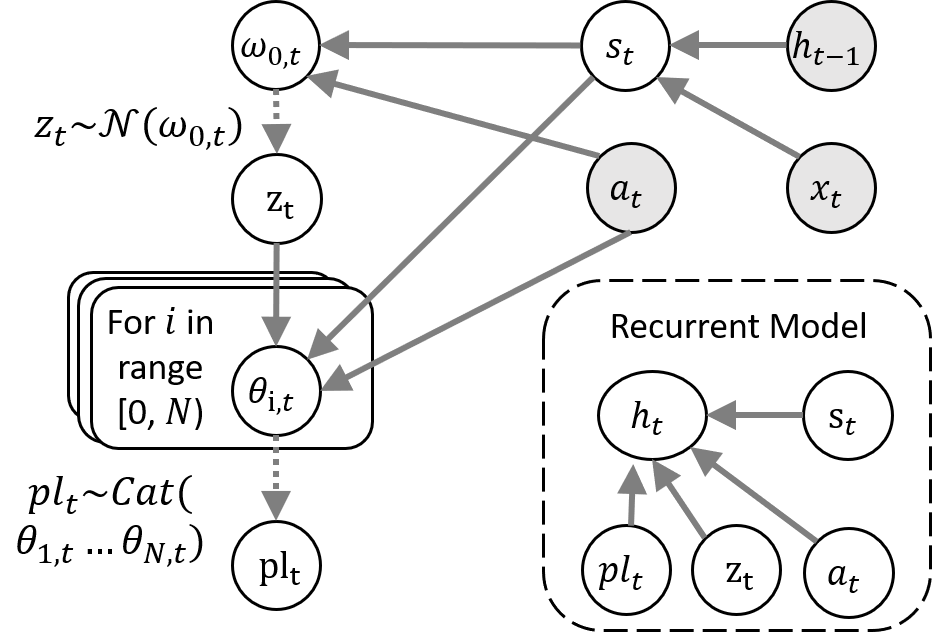
\includegraphics[width=0.8\columnwidth] 
    {./figures/hierarchical-model-graph.eps}
    \caption{Graphical illustration of our neural hierarchical model. Thick lines indicate logical function while dash line denotes stochastic dependence. The shaded nodes are given during generation. Our model applies hidden states $\hiddenstate_{t-1}$ of LSTM to capture the temporal dependence of  previously observed players and context variables. We represent the state as $\state_t \equiv (\features_{t},\hiddenstate_{t-1})$ and update the hidden states by $\hiddenstate_{t}=f(\features_{t},\action_{t},\latentvariables_{t},\hiddenstate_{t-1})$. $N$ is the number of players.
    } 
    \label{fig:hierarchical-model}
\end{figure} 
Following the above decomposition, Figure~\ref{fig:hierarchical-model} presents a graphical illustration of our hierarchical model.
Conditioning on game context ($\state_{t},\action_{t}$), the prior on the player representation $p(\latentvariables_{t}|\state_{t},\action_{t})$ follows a Gaussian distribution:
\vspace{-0.05in}
\begin{align}
    &\latentvariables_{t}|\state_{t},\action_{t}\sim p(\latentvariables_{t}|\state_{t},\action_{t}) \equiv \mathcal{N}(\boldsymbol{\GaussianParameters}_{0,t})\label{eqn:prior} \\
    &\boldsymbol{\GaussianParameters}_{0,t} :=\psi^{prior}[\psi^{\context}(\state_{t},\action_{t})]
\end{align}
\vspace{-0.01in}
\noindent where $\GaussianParameters_{0,t}\equiv[\boldsymbol{\mu}_{t,0},diag(\boldsymbol{\sigma}_{t,0})]$ denotes the parameters of the context-specific Gaussian prior. 
% \textcolor{red}{Should that be boldface $\mathbf{\mu}$ and $\mathbf{\sigma}$? Also, is the Gaussian isotropic (diagonal covariance) as you discussed in the Related work section?}
A neural network is trained to compute the parameter estimates by implementing 
%To derive those parameters, we implement 
a context function $\psi^{\context}$ to extract context features and a prior function $\psi^{prior}$ to compute $\boldsymbol{\GaussianParameters}_{0,t}$ from the extracted features. 
% The conditional prior of player embeddings is $\latentvariables_{t} | \state_{t},\action_{t} \equiv \expect_{\latentvariables_{i,t}\sim p(\latentvariables_{i,t}| \state_{t},\action_{t})}(\latentvariables_{i,t})$.

Given the game context and the sampled latent variables $\latentvariables_{t}$ from the context-specific Gaussian prior, %$(\state_{t},\action_{t})$, 
our model generates the label of the acting (or on-puck) player as follows:
\vspace{-0.05in}
\begin{align}
    \player_{t}| \latentvariables_{t}, \state_{t},\action_{t} &\sim Categorical(\BernoulliParameters_{1,t},\dots,\BernoulliParameters_{N,t})\\
    \BernoulliParameters_{\pindex,t}&:=\softmax\{\psi^{dec}[\psi^{z}(\latentvariables_{t}), \psi^{\context}(\state_{t},\action_{t})]\}
\end{align}
\vspace{-0.02in}
\noindent where neural function $\psi^{z}$ and $\psi^{c}$ extract features from latent variable $\latentvariables_{t}$ and context features respectively. The extracted features are sent to another decoder function $\psi^{dec}$. Given the decoder outputs, we apply a softmax function $\softmax$ to generate categorical parameters $\boldsymbol{\BernoulliParameters}_{t}$. $\BernoulliParameters_{\pindex,t}$ represents the probability of player $\pindex$ acting at time $t$. 

% These parameters are computed as follows: (1) A neural network implements the player embedding function $\psi^{z}$ to extract features from the player representations $\latentvariables_{t}$ (2) another neural network implements the context embedding function $ \psi^{\context}(\state_{t},\action_{t})$ to extract features from the game context. (3) The extracted features are input to a decoder function $\psi^{dec}$, whose outputs are normalizes to [0,1] by a softmax function $\softmax$. The normalized outputs are the parameters of a categorical distribution to model the acting players at time $t$.

Viewed as a predictive model, our neural hierarchical model solves a {\em re-identification task}~\cite{LaviRID2018}: identifying the currently acting player given the game context containing current observations and a history of events. 
% For example, a computer vision system may try to identify a player's jersey number from video footage. 
As Equation~\eqref{eq:player-factor} shows, this task captures the correlations between the identity of a player and what they do in which match contexts. To  achieve it, {\it the prior distribution $\prior(\latentvariables_{t}|\state_{t},\action_{t})$ forms a representation of game context, capturing which 
%the characteristics of 
players are likely to perform action $\action_{t}$ under state $\state_{t}$}. As a result, a promising representation for game context can be accurately mapped to the real acting player $\player_{t}$.
This observation inspires studying the performance of the neural hierarchical model for predicting the currently acting player (see the experiment in Section~\ref{subsec:identify-player}).


% By estimating the model parameters, we learn a contextualized player representation $\latentvariables_{i,t}|\player_{t}, \state_{t},\action_{t}$ = $\generation(\latentvariables_{i,t}|\GaussianParameters_{t,0},\state_{t},\action_{t})\generation(\GaussianParameters_{t,0}|\state_{t},\action_{t})$.


\subsection{Variational Inference}

% \textcolor{blue}{Maybe instead of naming it VAE, we should call it variational inference conditioning game context for the hierarchical model.} \textcolor{red}{Why not "hierarchical VAE"?}

We apply variational inference to derive an objective function for estimating the parameters of our hierarchical model. The inference is similar to that of Variational Auto-Encoder (VAE)~\cite{kingma2013auto}, because both models utilize a prior and approximate posterior on latent variables to define an approximate log-likelihood function for the observed data. 
% and fit them to a generator to predict the observation ($\player_{t}$ under our player embedding task) 2) define an approximate posterior on the latent variables and compute the parameters during inference. 
The main difference is that our hierarchical model conditions on the game context. In particular, the prior is learned to be a function of the game context, rather than a context-independent standard Gaussian distribution.

Figure~\ref{fig:model-struct} illustrates the inference process of our model. After observing the $\player_{t}$, the approximate posterior on a player embedding follows the equations:
\vspace{-0.03in}
\begin{align}
& \latentvariables_{t}|\player_{t} ,\state_{t},\action_{t} \sim \inference(\latentvariables_{t} |\player_{t} = \pindex,\state_{t},\action_{t}) \equiv \mathcal{N}(\boldsymbol{\GaussianParameters}_{\pindex,t})\label{eqn:approximate-posterior}\\
& \boldsymbol{\GaussianParameters}_{\pindex,t}:=\psi^{enc}[\psi^{\player}(\player_{t}=\pindex),\psi^{\context}(\state_{t},\action_{t})]
\end{align}

% Figure~\ref{fig:model-struct} illustrates the inference process of our model. After observing the $\player_{t}$, the approximate posterior on player embedding follows the equations:

% \begin{align*}
% & \latentvariables_{\player_{\pindex},t}| \player_{\pindex,t}, \state_{t},\action_{t} \equiv  \latentvariables_{\pindex,t}| \player_{\pindex,t}, \state_{t},\action_{t} \sim  \mathcal{N}(\boldsymbol{\GaussianParameters}_{\player_{\pindex},t})\\ 
% & \text{ where }  \boldsymbol{\GaussianParameters}_{\player_{\pindex},t}=\psi^{enc}[\psi^{\player}(\player_{\pindex,t}),\psi^{\context}(\state_{t},\action_{t})]
% \end{align*}

\noindent where we apply neural networks to implement 1) an observation function $\psi^{\player}$ that extracts features from  $\player_{t}$ (represented as an one-hot vector)
%and $\player_{\pindex,t}$ denotes the value in $\pindex^{th}$ dimension) 
2) a context function $\psi^{\context}$ that extracts features from game context ($\state_{t},\action_{t}$), and 3) an encoding function $\psi^{enc}$ that generates the parameters ($\boldsymbol{\GaussianParameters}_{\pindex,t}\equiv[\boldsymbol{\mu}_{\pindex,t},diag(\boldsymbol{\sigma}_{\pindex,t})]$) of an approximate Gaussian posterior.
% , with which we sample embeddings of individual players.
% We use 
% $\latentvariables_{\player_{\pindex},t}| \player_{\pindex,t}, \state_{t},\action_{t} \equiv  \latentvariables_{\pindex,t}| \player_{\pindex,t}, \state_{t},\action_{t}$
% % $\latentvariables_{\player,t} | \player_{t}, \state_{t},\action_{t} \equiv \expect_{\latentvariables_{\player_{\pindex},t}\sim q(\latentvariables_{\player_{\pindex},t}|\player_{\pindex,t}, \state_{t},\action_{t})}(\latentvariables_{\pindex,t})$ %. % \equiv \latentvariables| \player, \state,\action$ %
% %
% to emphasize that the code for the approximate posterior is associated with a specific observed player $\player_{t}$. 
{\it The approximate posterior $\inference(\latentvariables_{t} |\player_{t}=\pindex,\state_{t},\action_{t})$ naturally forms a
representation for current observed player $\player_{t}=\pindex$, from which we sample the latent variables and concatenate them into a context-specific embedding vector $\latentvariables_{t}$.} This real-valued vector can replace the one-hot player representation and facilitates downstream applications such as predicting expected goals or score differences (see Section~\ref{subsec:expected-goal} and~\ref{subsec:score-diff}). 
% Figure~\ref{fig:flow-chart} summarizes the entire learning process. 
% \todo{how do get an embedding vector out of the samples?}

\begin{figure}[t]
    \centering
    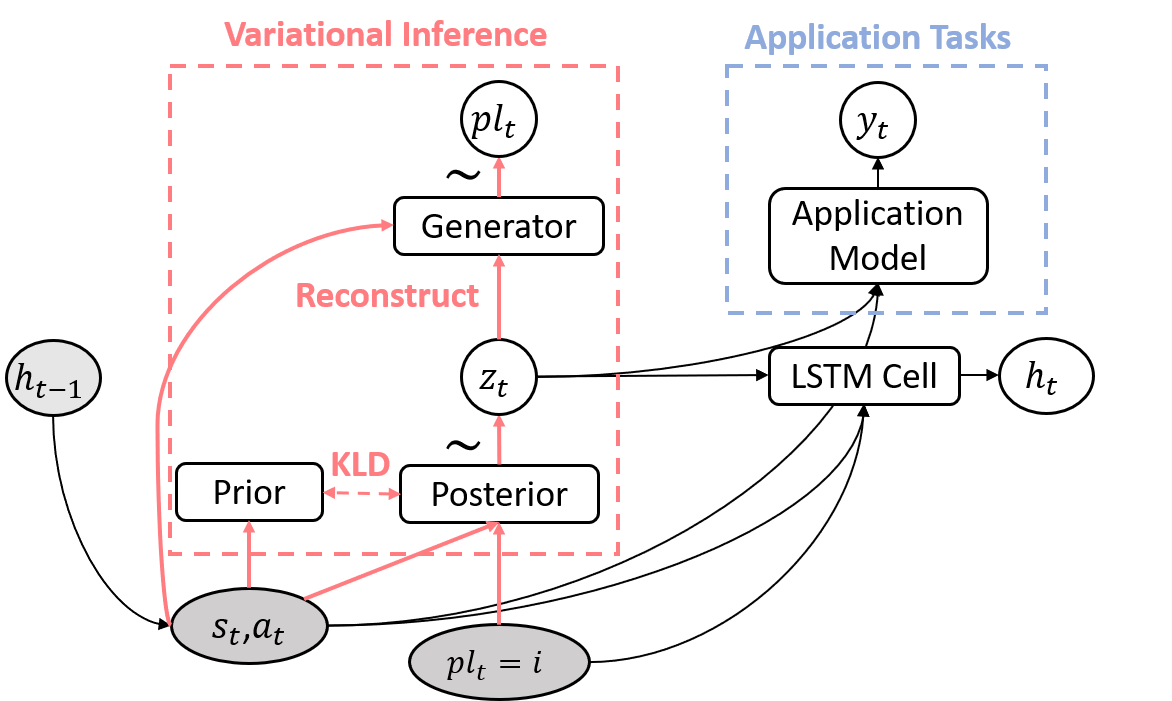
\includegraphics[width=1\columnwidth] 
    {./figures/variational-inference.eps}
    \caption{Learning the player representations to generate embeddings for application models. $y_{t}$ is the output of application model. The prior and the posterior respectively represent the Gaussian Prior and the approximate posterior of latent variables, with which the generator reconstructs $\player_{t}$. Red arrows indicate the process of variational inference. The shaded nodes are given during training.
    } 
    \label{fig:model-struct}
\end{figure} 
% \paragraph{Learning} 
Based on the time-wise variational lower bound~\cite{ChungKDGCB15}, the loss function for player embedding model is:
\vspace{-0.05in}
\begin{align} \label{eq:loss}
        &\sum_{t=1}^{T}\Big\{ KLD\Big[\inference(\latentvariables_{t} |\player_{t} = \pindex,\state_{t},\action_{t})||\prior(\latentvariables_{t}|\state_{t},\action_{t})\Big]-\\
        % &\expect_{\inference(\latentvariables_{\player,t} |\player_{t},\state_{t},\action_{t})}
        &\expect_{\latentvariables_{t}|\player_{t}=i,\state_{t},\action_{t}}
        \Big[\log\generation(\player_{t}|\latentvariables_{t},\state_{t},\action_{t}) -\lambda^{A}
        \mathcal{L}^{A}( \latentvariables_{t},\state_{t},\action_{t})\Big]
        \Big\} \nonumber
\end{align}
% \vspace{-0.1in}
\noindent where we add an application loss $\mathcal{L}^{A}$ with a parameter $\lambda^{A}$ to control its scale. This loss combines the gradient of the application models with the embedding inference. It allows simultaneously training the embedding model and the application model which not only significantly accelerates training but also dynamically incorporates player information into different downstream applications. 

\subsection{Discussion}~\label{sec:Interpretation}
\noindent We discuss the key motivations supporting our VHER model. 

\paragraph{Learning Contextualized Representations.} 
The behavior of sophisticated agents, like professional players, is highly sensitive to context. 
It is difficult to learn a fixed representation that can adequately describe a player's tendencies under every game context. 
Therefore, our VHER first learns a representation for game context (with the context-specific prior) and then asymptotically adjusts the posterior representation for individual players to each context during training.
% , rather than aiming to learn a single fixed prior representation.
The dynamically contextualized player representation significantly improves the robustness and comprehensiveness of embeddings, with which application models achieve better performance in the downstream tasks (see Section~\ref{subsec:expected-goal} and~\ref{subsec:score-diff}). 


\paragraph{Shrinkage Effect.} 
% A key motivation for our VHER model is a  shrinkage effect. 
%  We discuss show how our contextualized representation summarizes the available statistical information of a player. 
In a hierarchical model, shrinkage moves the posterior distribution for each player toward the prior mode. 
% A hierarchical model induces a shrinkage effect over parameters estimation which is commonly used in statistics to capture similarities among a group of individuals ~\cite{McCallum1998,kruschke2014doing}.  
% For example, previous parametric hierarchical models construct a separate parameter vector for each player~\cite{Murphybook12}.
% During parameters estimation, parameter vectors for each individual player are shrunk towards values representing the mode of their common prior.
Shrinkage estimators have strong statistical properties because they allow information to be transferred between the observations of different individuals. 
The shrinkage effect becomes stronger for players who share many statistical similarities under a game context, which %asymptotically 
draws their representations closer.
This naturally formalizes our intuition that {\em statistically similar players are assigned similar representations under similar game context.}
Our neural hierarchical model encourages such a shrinkage effect by minimizing the Kullback–Leibler Divergence (KLD defined in our loss function Equation~\eqref{eq:loss}) between posterior for each individual player and a context-specific prior. 

% shrinkage is achieved by estimating the individual players parameters using the posterior distribution over parameters drawn from a context-specific prior. 
% % The intuition motivating hierarchical models is that {\em statistically similar agents are assigned similar representations}.
% As Equation~\eqref{eq:loss} shows, 
% the loss function induces a shrinkage effect by regularizing the approximate posterior for each individual player towards a common prior $\prior(\latentvariables_{t}|\state_{t},\action_{t})$. The Conditional VAE, in fact, achieves a {\em joint} shrinkage effect where {\em statistically similar agents are assigned similar representations in similar contexts.} This is because we can interpret the prior distribution $\prior(\latentvariables_{t}|\state_{t},\action_{t})$ as a joint representation of the player's action and state: After training, state-action pairs that tend to feature the same players will be associated with similar prior distributions. In sum, we have described a parametric hierarchical model that generates dynamic context-aware player representations with a joint shrinkage effect for players, actions, and game states. 

\section{Empirical Evaluation}
In our experiments, we first evaluate the predictive performance of the embedding models under the task of identifying the acting player. To validate the generated player embeddings, we then incorporate them into the models for downstream application tasks following~\cite{PetersNIGCLZ18,AkbikBV18} and study the impact of embeddings on model performance.
The studied application tasks include 1) estimating expected goals and 2) predicting the final score difference. These are among the most challenging tasks in sports analytics %have been studied by many recent works
~\cite{ganguly2018problem}. 
% Figure~\ref{fig:model-struct} illustrates the process of feeding player embeddings into application models.

\subsection{Experiment Setting}
\paragraph{Training settings.}
Our model is implemented in Tensorflow (source code will be released after the anonymous reviewing). The dimension of the one-hot player vector $\player_{t}$ is 1,003 (the number of recorded players). The dimension of the player embedding as well as the dimension of parameters in Gaussian prior and posterior are set to 256. The max trace length of LSTM is set to 10 following previous work~\cite{Liu2018,littlestone}. The models are trained with Adam optimizer applying initial learning rate 1E-5\footnote{This paper uses many scientific notations, e.g., 1E-5=$1\times10^{-5}$.}.
%For robust evaluation results, we
We randomly divide the dataset containing 1,196 games into a training set (80\%), a validation set (10\%) and a testing set (10\%) and implement 5 independent runs. The resulting means and variances are reported.

\paragraph{Comparison models.}
% \textcolor{red}{In the remainder, we repeat quite a bit things like: this method uses game context, this  method is multimodal,etc. I think it would be better to make a table showing the methods and their properties. We could save space overall and it would help the reader understand our design.}

The design of our comparison models follows the ablation approach of removing different components from our full VHER system. 
We first remove the play history and train a Variational Hierarchical Encoder (\textbf{VHE}) to condition only on the current observations ($\features_{t},\action_{t}$). The second model is  
% hides context information from the prior. Instead, 
a traditional Conditional Variational Auto-Encoder (\textbf{CVAE})~\cite{WalkerDGH16} that applies a {\em context-independent} standard Gaussian distribution $\mathcal{N}(0,1)$ for a prior. We replace the variational model with a Deterministic Encoder (\textbf{DE}) \cite{ganguly2018problem} for player embedding. DE is trained as a regressor that directly maps the current game context to the acting player. Table~\ref{table:comparison-methods} shows a summary of the above models.
% \textcolor{red}{So is CVAE = VHER - Recurrence? Perhaps just call it VHE then.}
%To study the impact of player embeddings on 
In application tasks (Section~\ref{subsec:expected-goal} and \ref{subsec:score-diff}),
we compare the options of 1) applying one-hot player identities (\textbf{Pids}) to represent player information 2) adding no player information (\textbf{N/A}) to application models.

\begin{table}[htbp]
\addtolength{\tabcolsep}{-2pt} 
\resizebox{.5\textwidth}{!}{
\begin{tabular}{c|cccc}
\hline
 & \begin{tabular}[c]{@{}c@{}}Game \\ History\end{tabular} & \begin{tabular}[c]{@{}c@{}}Context- \\Specific Prior\end{tabular} & \begin{tabular}[c]{@{}c@{}}Multi-\\ Modal\end{tabular} & \begin{tabular}[c]{@{}c@{}}Continuous-\\ Value Embedding\end{tabular} \\ \hline\hline
DE & No & No & No & Yes \\
CVAE & No & No & Yes & Yes \\
VHE & No & Yes & Yes & Yes \\
VHER & Yes & Yes & Yes & Yes \\ \hline
\end{tabular}
}
\caption{A summary of compared embedding models. We omit Pids and N/A because they do {\it not} apply any embedding.}
\label{table:comparison-methods}
\end{table}

{\it Significance Test.} To assess whether embeddings of our VHER are significantly different from that of other models, we conduct a paired t-test over the embeddings computed with the testing dataset. The null hypothesis is rejected with p-values smaller than 1E-5 for all comparison models. 


\subsection{Predictive Performance of Embedding Models: On-Puck Player Identification}~\label{subsec:identify-player}
% Following~\cite{ganguly2018problem}, the player representations are learned under a task of predicting the acting player given the game context, so 
This experiment studies the performance of embedding models as predictive models under the embedding task: identifying the acting player. We compare our VHER model to seven baselines including 1) directly applying a LSTM to model the game history and identify the acting player without a player embedding and 2) three embedding models: DE, CVAE, and VHE, which do not consider game history during training. To make a fair comparison, we also consider providing these three methods with information about the recent play history by {\it constraining (CSTR)} their predictions to a group of recently acting players: the current on-puck player (the correct answer) and the players that have possessed the puck in the previous 10 (the trace length of LSTM) steps during testing.
% ~\textcolor{blue}{more explain here?} 
% In contrast, our VHER method has to predict the current on-puck player from the full set of 1003 players, \todo[color=red]{Galen: is this true?} \todo[color=blue]{guess we don't have to emphasize it.} and has to learn to remember recently observed players. 

% and study the influence of incorporating play history, we consider two also evaluate the options of 1) directly applying a LSTM to identify the acting player. 2) Selecting on-puck candidates from a group of recently acting players, which  contains the current on-puck player (right answer) and the players that have possessed the puck in the previous 10 (LSTM trace length) steps during testing.  
% To assess alternative ways of including player information, we also experiment with the options of including players' pre-game cumulative box score (see table~\ref{table:feature-of-dataset}) into game context. \todo{what is LSTM method?}

\begin{table}[htbp]
\addtolength{\tabcolsep}{-1pt} 
\centering
    \begin{tabular}{c|cc}
    \hline
     \multirow{2}{*}{\begin{tabular}[c]{@{}c@{}}Prediction\\ Method\end{tabular}} & \multicolumn{2}{c}{Performance} \\ \cline{2-3}
     & Accuracy & Log-Likelihood \\ \hline \hline
    DE & 9.40 \% $\pm$ 3.06E-3 \% & -17.42 $\pm$ 2.23E-1 \\
    CVAE & 10.40 \% $\pm$ 6.01E-2 \% & -4.92 $\pm$ 6.03E-6  \\
    VHE & 11.18 \% $\pm$ 2.71E-3 \% & -4.91 $\pm$ 2.74E-5  \\\hline
    DE-{\it CSTR} & 27.32 \% $\pm$ 8.56E-3 \% & -17.42 $\pm$ 2.23E-1 \\
    CVAE-{\it CSTR}&  28.61\% $\pm$ 2.07E-2 \% & -4.92 $\pm$ 1.38E-6 \\
    VHE-{\it CSTR} & 31.04\%  $\pm$ 3.45E-2 \% & -4.91 $\pm$ 3.25E-6  \\\hline
    LSTM & 36.49\% $\pm$ 2.21E-4 \% & -3.10 $\pm$ 2.80E-4\\
    VHER & \textbf{48.36} \% $\pm$ 1.18E-3 \% & \textbf{-2.09} $\pm$ 2.36E-3\\ \hline
    \end{tabular}
    \caption{Results for the on-puck players identification.}
    \label{table:exp-pid}
\end{table}



Table~\ref{table:exp-pid} shows the  results for acting player identification. Predictions from DE have a substantially smaller log-likelihood than the other methods, because it is trained as a standard regression model: the DE objective minimizes the distance between a single prediction and the ground truth. This method, however, will fail if the output space is multimodal.
To handle it, variational models compute multiple isotropic Gaussian priors (see Equation~\eqref{eqn:prior}) on the latent variables, which creates disentangled representations for each player, and thus facilitates the modeling of multiple modes.
Therefore CVAE manages to improve the log-likelihood, but its performance is still limited by the lack of game context. By applying a context-specific prior, VHE achieves a small improvement. 
We also find constraining the candidate players to the group of recent on-puck players improves the performance of DE, CVAE, and VHE. However, the LSTM recurrent memory extracts still more useful information from the match history even without player embeddings. 
Our VHER incorporates play history into both variational inference and player embeddings. This combination allows
% \textcolor{red}{Does CVAE or VHE include a common prior and shrinkage effect as well? See question above.}
{\em VHER to substantially increase both the prediction accuracy and the log-likelihood over other comparison methods.}
% \textcolor{red}{OS: very nice result! We may not need such a detailed discussion of the results for different methods.}\textcolor{blue}{but we don't such discussion in the following experiments.}
% We also find including the box score will further improve the performance. This is because the box-scores provide a strong prior for identifying the acting player. 
% The model can easily determine the ability of a player without looking at game data. \textcolor{red}{Do you mean "identity" or "ability". Also, this does not seem to be easy for the CVAE. Kind of strange. Maybe omit this sentence}



% \begin{table}[htbp]
%     \centering
%     \addtolength{\tabcolsep}{-3pt} 
%     % \resizebox{.5\textwidth}{!}{
%         \begin{tabular}{c|cccc}
%         \hline
%         \multirow{2}{*}{\begin{tabular}[c]{@{}c@{}}Embed\\ Method\end{tabular}} & \multicolumn{4}{c}{Performance without Box-Scores} \\ \cline{2-5}
%         & P & R & F1 & LL \\ \hline\hline
%         % $\emptyset$ 
%         N/A & 0.12 & 0.84 & 0.21 & -0.64 \\
%         Pids  & 0.08 & 0.65 & 0.14 & -0.64\\
%         DE  & 0.29 & 0.91 & 0.44 & -1.69 \\
%         CVAE  &  0.34 & 0.95 & 0.50 & -1.61 \\
%         VHE & 0.33.33E-5 & 0.95 & 0.50 & -1.55 \\
%         VHER  & 0.40 & 0.84 & 0.54 & -0.96 \\ \hline
%         \end{tabular}
%         % }
%         \caption{Results for predicting the Expected Goal. The evaluation metrics include Precision (P), Recall (R), F1-score and Log-Likelihood (LL). }
%         \label{table:exp-eg}
% \end{table}
% \begin{table}[htbp]
%     \centering
%     \addtolength{\tabcolsep}{-3pt} 
%     % \resizebox{.5\textwidth}{!}{
%         \begin{tabular}{c|cccc}
%         \hline
%         \multirow{2}{*}{\begin{tabular}[c]{@{}c@{}}Embed\\ Method\end{tabular}} & \multicolumn{4}{c}{Performance with Box-Scores} \\ \cline{2-5}
%         & P & R & F1 & LL \\ \hline\hline
%         % $\emptyset$ 
%         N/A & 0.10 & 0.78 & 0.18 &-0.64 \\
%         Pids  & 0.09 & 0.52 & 0.15 & -0.56\\
%         DE  & 0.25 & 0.96 & 0.40 & -2.40 \\
%         CVAE  & 0.35 & 0.92 & 0.51 & -1.41 \\
%         VHE & 0.36 & 0.92 & 0.51 & -1.37 \\
%         VHER  & 0.41 & 0.82 & 0.55 & -0.64 \\ \hline
%         \end{tabular}
%         % }
%         \caption{Results for predicting the Expected Goal. The evaluation metrics include Precision (P), Recall (R), F1-score and Log-Likelihood (LL). }
%         \label{table:exp-eg}
% \end{table}

\subsection{Application 1: Expected Goals Estimation}\label{subsec:expected-goal}

In this section, we validate the player embeddings in a practical task of estimating the Expected Goal (XG). 
An XG metric weights each {\it shot} by its chance of leading to a goal and ignores other actions. To see if the embeddings improve the accuracy of XG estimates, we sample the player embedding $\latentvariables_{t}$ from the learn player representation $\inference(\latentvariables_{t} |\player_{t} ,\state_{t},\action_{t})$ (cf. Figure~\ref{fig:model-struct}). 
% for the acting player $\player_{t}$ (cf. Figure~\ref{fig:model-struct}). \todo[color=red,inline]{What is the embedding $\latentvariables_{t}$ exactly? The mean of the posterior?}
At time $t$, we 
input $\state_{t},shot_{t},\latentvariables_{t}$ to the application model, which is trained to generate 1 if a goal is scored after the player $\player_{t}$ makes the shot and 0 otherwise. Our {\em application model} is a LSTM that generates the expected goal given the inputs. Our dataset provides ground-truth labels for whether a given shot led to a goal. 
% The model is trained with the game context for action shot in our NHL dataset and we supervise the training by whether the shot will lead to a goal in real games. 
Since only a few shot attempts lead to a goal ($<$3.9\%), the training data is highly imbalanced.
% , which will encourage the model to label all the shots as 0, in order to %improve the overall prediction accuracy. 
We, therefore, employ a resampling method~\cite{good2006resampling}, so successful and failed shots (e.g. blocked or missed) occur equally often during training.

\begin{table}[!htbp]
    \centering
    \addtolength{\tabcolsep}{-1.5pt} 
    \resizebox{.5\textwidth}{!}{
        \begin{tabular}{c|ccc}
        \hline
        \multirow{2}{*}{\begin{tabular}[c]{@{}c@{}}Embed\\ Method\end{tabular}} & \multicolumn{3}{c}{Performance} \\ \cline{2-4}
        & Precision & Recall & F1-score \\ \hline\hline
        % $\emptyset$ 
        N/A &  0.12 $\pm$ 1.75E-4 & 0.79 $\pm$ 9.46E-4 & 0.21 $\pm$ 4.26E-4 \\
        Pids  & 0.09 $\pm$ 1.62E-4 & 0.62 $\pm$ 2.52E-3 & 0.15 $\pm$ 4.20E-4 \\
        DE  & 0.30 $\pm$ 1.26E-4 & 0.92 $\pm$ 4.21E-4 & 0.45 $\pm$  1.87E-4\\
        CVAE & 0.32 $\pm$ 1.05E-4 & 0.94 $\pm$ 1.56E-4 & 0.48 $\pm$ 1.65E-4 \\
        VHE & 0.33 $\pm$ 5.33E-5 & \textbf{0.95} $\pm$ 8.72E-5 & 0.49 $\pm$ 8.29E-5  \\
        VHER  & \textbf{0.40} $\pm$ 4.75E-4 & 0.84 $\pm$ 1.81E-4 & \textbf{0.54} $\pm$ 2.97E-4 \\ \hline
        \end{tabular}
        }
        \caption{Results for predicting the Expected Goal using a LSTM with different methods of including player information. 
        % The evaluation metrics include Precision (P), Recall (R) and F1-score.
        }
        \label{table:exp-eg}
\end{table}
\vspace{-0.1in}
% We refer to a neural net for the validation task as the validation model. Our validation model is an LSTM that is given the play history, combined with three comparison methods of including current-player information: 1) our dense VHER embeddings, 2) directly inputting one-hot player ids (Pids), 3) no player information. 
% (e.g. VHER) and with Dense layers otherwise (e.g. Encoder and CVAE). 
% To investigate the advantage of continuous-value embedding vectors for players, we also evaluate comparison methods including apply no player information ($\emptyset$) and directly inputting player ids (Pids) into the validation model.
% To train the validation model, we utilized the game context for action shot recorded in our NHL dataset and supervise the training by whether the shot will lead to a goal in real games. However, considering that most of the shots will not score any goals, the training data is highly imbalanced.
% , which will encourage the model to label all the shots as 0, in order to %improve the overall prediction accuracy. 
% We handle the imbalance with a resampling method~\cite{good2006resampling} so that equal numbers of success and failed shots are included in the training dataset. 

Table~\ref{table:exp-eg} shows the results on the testing set.\footnote{We do not report the AUC metric because it over-emphasizes the negative samples and does not discriminate among methods.} %, due to the imbalanced data.}.
Without including any player information (N/A), predictions have large recall but very limited precision, because the model prefers labeling many shots as goals. On this dataset, achieving high precision is a difficult challenge. 
%, but most of the predictions are incorrect. 
% This problem has not been alleviated after 
Adding the pids to the input does not improve precision, which shows it is hard to utilize the player information with only a sparse one-hot label. 
%Providing more useful player information, 
The DE player embedding substantially improves both precision and recall. 
% deterministically maps the player information into a dense player embedding vector. 
CVAE and VHE achieve some improvement with the variational auto-encoder, but it is limited due to the lack of play history information.
% further model the embedding with the latent variables, but they achieve only limited improvement. A common problem for the above embedding methods is the absence of play history during training. 
VHER applies a recurrent model to include previous game contexts and player information, which brings a big improvement in precision and a loss of recall. {\em VHER achieves the best precision and F1-score.}
% \textcolor{red}{this sounds as if adding recurrence to DE during embedding would fix most of the problems. Something for future work?}
% We also experiment applying box score \textcolor{blue}{more results to be include}

%would be interesting to know the accuracy on unprocessed test set data

% \begin{table}[htbp]
% \begin{tabular}{ccccc}
% \hline
% Model & TP & FP & TN & FN \\ \hline
% LSTM & 572 & 3,389 & 13,109 & 136 \\
% LSTM+Pid & 489 & 4,269 & 12,229 & 219 \\
% Encoder+Dense & 360 & 2,278 & 14,220 & 348 \\
% CVAE+Dense & 670 & 2,073 & 14,425 & 38 \\
% CVRNN+LSTM & 618 & 609 & 15,889 & 90 \\
% CVRNN+LSTM+Box & 608 & 405 & 16,093 & 100 \\ \hline
% \end{tabular}
% \caption{The detailed results of Expected Goal experiment.}
% \end{table}

\subsection{Application 2: Score Difference Prediction}\label{subsec:score-diff}
Dynamic Score Difference Prediction (DSDP) is a recently proposed task~\cite{ganguly2018problem} that requires to predict the final score difference $\scorediff(T)$ under a game context ($\state_{t},\action_{t}$) where $t$ runs from 0 (game starts) to $T$ (game ends). 
In preliminary experiments, we observed that traditional supervised learning methods suffer a large training variance (especially in the early game when there have multiple possible outcomes).
%, and thus fail to converge. 
To exploit the temporal dependencies between score differences at successive times, we apply reinforcement learning; specifically the temporal difference method Sarsa prediction~\cite{sutton2018reinforcement}. Sarsa learns a Q-function for a generic home/away team to estimate the expected cumulative goal scoring: $Q_{\team}(\state_{t},\action_{t})= \expect(\sum_{\tau=t}^{T}\goal_{\team,\tau})$ where $\team=\home/\away$ and $\egoal_{\team}$=1 if the team scores at $t$ and 0 otherwise. Given Q-functions, the final Score Difference Prediction (SDP) is given by % \begin{equation}
    $SDP(\state_{t},\action_{t}, \player_{t})= Q_{\home}(\cdot)-Q_{\away}(\cdot) + \scorediff(t)$.
% \end{equation}
Our {\em application model} is a DRQNN~\cite{littlestone} that computes the Q-functions. The inputs are state $\state_{t}$, action $\action_{t}$ and the embedding $\latentvariables_{t}$ (sampled from player representation $\inference(\latentvariables_{t} |\player_{t} ,\state_{t},\action_{t})$) for the acting player $\player_{t}$. 

Figure~\ref{fig:temporal-diff} illustrates the mean and the variance of the absolute error ($ |SDP(\state_{t,m},\action_{t,m}, \player_{t,m})-\scorediff(T,m)|$, where $m\in[0, M]$ and $M$ denotes the number of testing games), at each time step $t$. The plot shows a larger difference between real and predicted SDs at the beginning of a game, but the mean and variance of the difference become smaller towards the game end. Among the evaluated embedding methods, our {\em VHER (the black line) manages to generate the player representations that lead to the most accurate predictions.} We also find that the accuracy advantage is strongest towards the early game, especially compared to the N/A and pids. This indicates that an informative player representation can significantly alleviate the difficulty of predicting multiple outcomes in the early game. We also report the average Mean Absolute Error (MAE) over all game times in Table~\ref{table:avg-diff}. The VHER embeddings lead to the lowest average MAE. 
% \textcolor{red}{comments from the sportlogiq guys. 1) Pregame about half the games have score diff 1 or -1. If you say 0 for all games at time 0, the average error would be 1.8. So it's strange that the baseline methods are above 2.0 at the beginning.} \textcolor{red}{2) Another comment was that they would like to see the evolution of score difference predictions (rather than errors). This could be more directly checked against game understanding and calibration stats.} \textcolor{red}{3) Why are the errors not close to 0 towards the game end? Is current score differential one of the features? Are you including overtime games? Even including overtime games the error at game end should be something like 0.2 not 0.5.}
\vspace{-0.3in}
\begin{figure}[htbp]
\hspace{-0.15in}\begin{minipage}[b]{.5\columnwidth}
\centering\
\subfloat{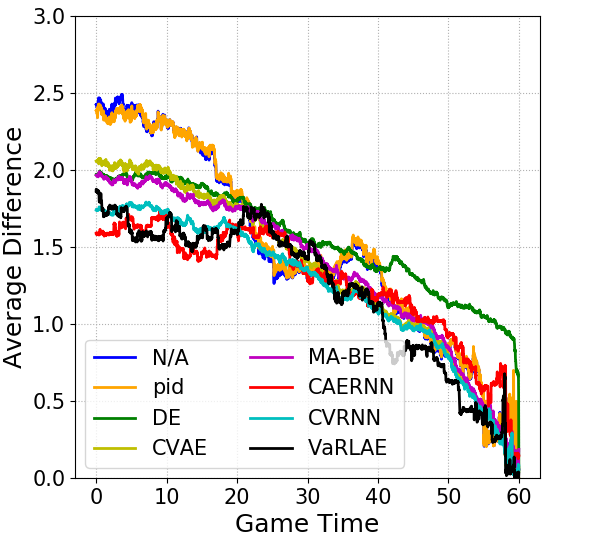
\includegraphics[scale=.32]{figures/temporal-absolute-difference-plot.png}}
\end{minipage}%
\hspace{0.15in}\begin{minipage}[b]{.5\columnwidth}
\centering
\subfloat{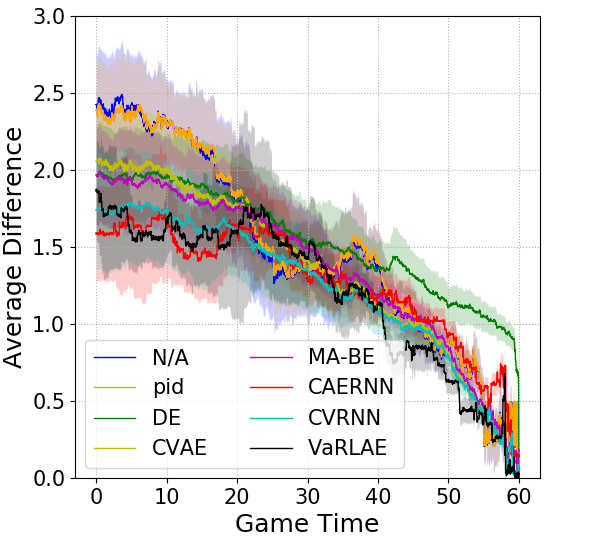
\includegraphics[scale=.32]{figures/temporal-absolute-difference-shadow-plot.png}}
\end{minipage}
\vspace{-0.2in}
\caption{Temporal illustrations of the differences between predicted score differences and final score differences applying different embeddings. We report the plot with the mean of differences (left) and the plot with the mean$\pm$variance of differences (right).} 
\label{fig:temporal-diff}
\end{figure}
\vspace{-0.1in}
\begin{table}[htbp]
    \centering
    \begin{tabular}{c|c|c|c}
    \hline
    Method  &  MAE &  Method  &  MAE\\\hline\hline
    N/A & 1.55 $\pm$ 0.35 & CVAE & 1.52 $\pm$ 0.30\\
    Pid & 1.56 $\pm$ 0.32 & VHE & 1.49 $\pm$ 0.29\\
    DE & 1.48 $\pm$ 0.24 & VHER & \textbf{1.32} $\pm$ 0.27\\ \hline
    \end{tabular}
    \vspace{-0.1in}
    \caption{The average differences between predicted and final score differences over the entire game times for all testing games.}
    \label{table:avg-diff}
\end{table}
\vspace{-0.2in}
% \begin{table}[]
%     \centering
%     \begin{minipage}[b]{.5\columnwidth}
%         \begin{tabular}{c|c}
%         \hline
%         Method  &  MAE \\\hline\hline
%         N/A & 1.55 $\pm$ 0.35 \\
%         Pid & 1.56 $\pm$ 0.32 \\
%         DE & 1.48 $\pm$ 0.24 \\ \hline
%         \end{tabular}
%     \end{minipage}%
%     \begin{minipage}[b]{.5\columnwidth}
%         \begin{tabular}{c|c}
%         \hline
%         Method  &  MAE \\\hline\hline
%         CVAE & 1.52 $\pm$ 0.30 \\
%         VHE & 1.49 $\pm$ 0.29 \\
%         VHER & \textbf{1.32} $\pm$ 0.27 \\\hline
%         \end{tabular}
%     \end{minipage}
%     \caption{The average differences between predicted score and final score differences applying different embeddings.\textcolor{red}{Why not make this table two-column?}}
%     \label{table:avg-diff}
% \end{table}


% \subsection{Estimate the Next-Goal Scoring Probability} 
% % \textcolor{blue}{ Previous evaluations work only on action shot, and current evaluations are for all actions.}
% We compute Q values to estimate the probability of scoring the next goal within different states of a NHL game. 
% Unlike the previous expected goal which considers only the action shot, a Q-function estimates the influence of every actions and their states on scoring the next goal. 
% To learn the Q function, we follow~\cite{Liu2018} and divide a NHL game into {\bf goal-scoring episodes}, so that each episode 1) starts at the beginning of the game, or immediately after a goal, and 2) terminates with a goal or at the end of the game. 
% % A goal-scoring episode contains sufficient information about both offensive and defensive movements of players in home and away team.
% In a goal-scoring episode, the Q values estimated the expected probability that the home resp. away team {\em scores the goal at the end of the current goal-scoring episode} ($\egoal_{\home}=1$ resp. $\egoal_{\away}=1$), or neither team scores ($\egoal_{\none}=1$), so $ Q_{\team}(\state_{t},\action_{t}, \player_{t}) = P(\egoal_{\team}=1|\state_{t},\action_{t}, \player_{t})$.
% % The estimated Q values offer a natural approach to evaluate a player current performance by measuring its influence to score the next goal. 
% To compute those Q values, we implement the validation model (in Figure~\ref{fig:model-struct}) with a Deep Recurrent Q-learning Neural Network (DRQNN)~\cite{littlestone} and the input at each running step $t$ contain state $\state_{t}$, action $\action_{t}$ and the embedding $\latentvariables_{t}$ for the current acting player $\player_{t}$.
% % DRQNN constructs a recurrent neural network to fit the game history data at every time step $t$ and apply Temporal Difference (TD) learning to train the Q function, whose values both remember game history and look ahead to the next goal. 

% We evaluate how well our learned Q-function fits the observed next-goal scoring frequencies under different discrete game contexts.
% Our approach to defining the game context is 
% % To define empirical event frequencies, 
% dividing the continuous environment variables $\features_t$ into discrete bins representing a type of game context.
% To calculate empirical visiting frequencies of bins, we assign an observed state $\state_{t}$ to a bin according to the values of three discrete {\em context features} in the last observation: Manpower (Short Handed (SH), Even Strength (ES), Power Play (PP)), Goal Differential ($\leq -3$, -2, -1, 0, 1, 2, $\geq 3$) and Period (1, 2, 3). The total number of bins is $3\times 8 \times 3 =72$. This partition has two advantages. 1) The context features are well-studied and important for soccer experts~\cite{decroos2018action}, so the model predictions can be checked against domain knowledge. 
% %\textcolor{Orange}{For instance, a manpower advantage increases the scoring chances for the home team more than it increases them for the away team.} 
% 2) The partition covers a wide range of match contexts, and each bin aggregates a large set of play histories. If our model exhibits a systematic bias, 
% %in some match context, 
% the aggregation should amplify it and become detectable. 

% Given the set of bins where each bin $\bin$ contains a total of $|\bin|$ states, the empirical and estimated scoring probabilities for each bin are defined as follows: 
% \begin{itemize}
%     \item { \it Empirical Scoring Probabilities (Emp-SP) }: for each observed state $\state$, we set $\egoal^{obs}_{\team}(\state) = 1$ if the observed episode containing state $\state$ ends with a goal by team $\team = \home,\away$ or neither ($\team = \none$). Then $\Qobs{\team}{\bin} = \frac{1}{|\bin|}\sum_{\state \in \bin} \egoal^{obs}_{\team}(\state)$
%     \item { \it Estimated Scoring Probabilities (Est-SP)}: we apply the validation model to estimate a Q value for each observed sequence and average the resulting estimates to compute the estimated scoring probabilities : $\Qbin{\team}{\bin} = \frac{1}{|\bin|}\sum_{\state \in \bin} \Qmodel{\team}{\state}{\action}$ 
% \end{itemize}

% We compute both the Mean Average Value and the KL-Divergence between the Empirical and the Estimated Scoring Probabilities for a {\it total} bin containing all the states and report their average value in table~\ref{table:next-goal-results}.

% \begin{table}[!htbp]
% \centering
%     \begin{tabular}{c|cc}
%     \hline
%      \multirow{2}{*}{\begin{tabular}[c]{@{}c@{}}Embed\\ Method\end{tabular}} & \multicolumn{2}{c}{Performance} \\ \cline{2-3}
%      & MAE & KLD \\ \hline \hline
%     N/A & 0.1498 $\pm$ 7.63E-4 & 0.02386 $\pm$ 8.52E-5 \\
%     Pids & 0.1545 $\pm$ 6.27E-4  & 0.02474 $\pm$ 7.35E-5 \\
%     DE & 0.1048 $\pm$ 2.01E-3 & 0.07106 $\pm$ 3.13E-3 \\
%     CVAE & 0.0906 $\pm$ 2.09E-3  & 0.00899 $\pm$ 6.70E-4 \\
%     VHE & 0.0870 $\pm$ 2.16E-3 & 0.01112 $\pm$ 7.95E-4\\
%     VHER & 0.0517 $\pm$ 7.26E-4 & 0.00272 $\pm$ 5.21E-6  \\ \hline
%     \end{tabular}
%     \caption{Results for estimating the next goal scoring probability.}
%     \label{table:next-goal-results}
% \end{table}

% \begin{table*}[!htbp]
% \centering
% \begin{tabular}{ccc|c|ccc|cccccc}
% \hline
% \multicolumn{4}{c|}{Environment Features} & \multicolumn{3}{c|}{VHER Values} & \multicolumn{6}{c}{MAE / Log-Likelihood} \\ \hline
% MP & GD & P & Count & Home & Away & End & VHER & HER & CVAE & DE & Id & N\textbackslash{}A \\ \hline \hline
%  SH & 1 & 3 & 33 & 0.3832 & 0.4087  &  &  &  &  &  &  \\
%  SH & 0 & 3 & 55 & 0.3968 & 0.4297  &  &  &  &  &  &  \\
%  SH & -1 & 3 & 56 & 0.3874 & 0.4156  &  &  &  &  &  &  \\
%  ES & 1 & 3 & 2232 & 0.4371 & 0.3478  &  &  &  &  &  &  \\
%  ES & 0 & 3 & 2550 & 0.438 & 0.3489  &  &  &  &  &  &  \\
%  ES & -1 & 3 & 2090 & 0.4453 & 0.3540 &  &  &  &  &  &  \\
%  PP & 1 & 3 & 236 & 0.5211 & 0.3052  &  &  &  &  &  &  \\
%  PP & 0 & 3 & 170 & 0.5334 & 0.3104  &  &  &  &  &  &  \\ 
%  PP & -1 & 3 & 157 & 0.5254 & 0.3072  &  &  &  &  &  &  \\ 
%  \hline
% \end{tabular}
% \caption{Calibration Results.}
% \end{table*}


% % \begin{table*}[!htbp]
% % \centering
% % \begin{tabular}{ccc|c|cc|cccccc}
% % \hline
% % \multicolumn{4}{c|}{Environment Features} & \multicolumn{2}{c|}{VHER Values} & \multicolumn{6}{c}{MAE / Log-Likelihood} \\ \hline
% % MP & GD & P & Count & Home & Away & VHER & HER & CVAE & DE & Id & N\textbackslash{}A \\ \hline \hline
% %  &  &  &  &  &  &  &  &  &  &  &  \\
% %  &  &  &  &  &  &  &  &  &  &  &  \\ \hline
% % \end{tabular}
% % \caption{Calibration Results.}
% % \end{table*}
% % \begin{table}[t]
% % \centering
% %     \begin{tabular}{c|cc}
% %     \hline
% %      \multirow{2}{*}{\begin{tabular}[c]{@{}c@{}}Embed\\ Method\end{tabular}} & \multicolumn{2}{c}{Performance (With Box-Scores)} \\ \cline{2-3}
% %      & MAE & KLD \\ \hline \hline
% %     N/A & 4.19E-2 & 1.34E-2 \\
% %     Pids & 4.17E-2 & 1.439E-2\\
% %     DE &  &  \\
% %     CVAE & 6.63E-2 & 5.89 E-2\\
% %     VHE & 4.11E-2 &  1.63E-2\\
% %     VHER & 1.42E-2 &  1.11E-3  \\ \hline
% %     \end{tabular}
% % \end{table}

\section{Conclusion}
Capturing what players have in common and how they differ is one of the main concerns of sports analytics. 
In this work, we propose a novel VHER model to generate a deep contextualized player representation for Hockey players.  VHER learns a context-specific prior over player representations and derives posterior representation for each acting player sharing the common prior. This hierarchical structure induces a shrinkage effect formulating the intuition that similar players are mapped to similar representations in similar match contexts. We sample player embeddings from the representation distribution and validate them in the tasks of identifying the acting player, estimating the expected goals and predicting the final score difference.
A direction of future work is developing a multi-agent embedding model for team sports with complex game context (e.g. ice hockey and soccer).
Given an advanced dataset having full observability of on-court players, the model can learn the interactions between multiple players and generate embeddings for different lineups.


\bibliographystyle{named}
\bibliography{master}


% \appendix

% \subsection{Contextual Features for Embedding}
% \oliver{this is an interesting discussion. It's nice in general. It does not directly address whether we want a single embedding or a conditional one. For example, one could view a player as a mapping from context to actions.}



% \textcolor{blue}{We could somehow introduce a new language to describe the player embedding features. Like the SPADL, how about Player Embedding Language for Ice-hockey (PELI)}
% Please introduce the box scores here.
% Our embedding language should consider the following points:
% \begin{itemize}
%     \item Actions: In general, players are only specialists of a certain number of actions. For example, wingers will master the shooting and passing skill while defense men know how to block the attackers and check them from the puck. Our embedding should modeling a player's ability of performing different actions. 
%     \item Temporal features: Our embedding considers the game time and action duration, because 1) a player will behave diversely at different time of a game. For instance, some players requires a few minutes to heat up in the early game while some players can bring immediate contribution when the coach places him on ice. 2) The time spent to complete an action reflects the skill of a player. An example is that the player's ability of making quick shot will determine if he can catch the sudden opportunity to score a goal.
%     \item Spatial features: Location of players, velocity of the puck and distance from the goal will significantly influence a player performance. It is why, to increase scoring probability, most of players choose to shot near their opponent's goal. However, there are still some players who are skilful at making long shot. Our embedding should consider these difference.
%     \item Gaming Features: Manpower situation and goal difference affects a player decision. A few scores behind and the short-handed situation will testify a player's ability to handle high pressure. Another phenomenon that is worth modeling is the home advantage. Players are like to perform well in their home city with their fans~\cite{swartz2014}.
%     \item Pre-game Box Score: Our embedding contains the current season pre-game box score of each player (except Goalies, as unlike skaters, they apply another stats system.\textcolor{blue}{I don't know, maybe we should include the goalies.}). We add up the game-by-game player stats before a target game. In this sense, we assume zero prior knowledge about the results of the game. \oliver{???}
% \end{itemize}
% \oliver{we could also have considered which player acted previously}

% \section{Our Method}



% \subsection{Compute Player Embedding with CVRNN}
% In this section, we  introduce the Conditional Variational Recurrent Neural Network (CVRNN), with which we learn the conditional embeddings for ice hockey players.

% The CVRNN follows a recurrent structure and defines a Conditional Variational Auto-Encoder (CVAE) at every time step $t$. 
% Unlike traditional VAE which generates a set of latent random variables to capture only the variation of current observation
% % (one-to-one mapping $q(\latentvariables_{t}|\player_t$))
% , CVAE conditions the entire generation process on the another set of environment variables $\context_{t}$.
% % and achieves a many-to-one mapping $q(\latentvariables_{t}|\player_t,\context_t)$.
% In the scenario of ice hockey, the current observation is the id of current on-the-ball player $\player_{t}$ and latent variables $\latentvariables_{t}$ represent the embedding of $\player_{t}$. We condition the generation process of $\latentvariables_{t}$ on the player action $\action_{t}$, current game state $\state_{t}$, play history $\hiddenstate_{t-1}$ and the accumulative boxscore (pre-game) of embedded player $\boxscore_{\player_{t}}$ which reasonably features the current game environment: $\context_{t} = (\state_{t},\action_{t},\hiddenstate_{t-1},\boxscore_{\player_{t}})$. 
% % In the following, 
% We split the the generation process into encoding and decoding and explain how CVRNN learns to generate the player embeddings.


% \subsubsection{Encoding}

% {\em Model Definition.}
% Encoding is where CVRNN generates the player embeddings.
% At time step $t$, CVRNN generates two set of latent variables: $\latentvariables_{\player,t} $ and  $\latentvariables_{0,t}$. $\latentvariables_{\player,t} $ assumes that we know the id of current on-the-ball player $\player_{t}$ while $\latentvariables_{0,t}$ does not know $\player_{t}$. We present the process of generating both latent variables and explain the idea of applying $\latentvariables_{0,t}$ to learn the embedding. 


% Latent variables $\latentvariables_{\player,t} $ are sampled from a conditional posterior $\inference(\latentvariables_{\player,t} |\player_{t},\context_{t})$:
% \begin{align*}
% \latentvariables_{\player,t} & \sim \inference(\latentvariables_{\player,t} |\player_{t},\context_{t}) \\ 
% \inference(\latentvariables_{\player,t} |\player_{t},\context_{t}) & = \mathcal{N}(\mu_{\latentvariables,t},diag(\sigma^{2}_{\latentvariables,t}))\\
% [\mu_{\latentvariables,t},\sigma_{\latentvariables,t}]&=\psi^{enc}(\psi^{\player}(\player_{t}),\psi^{\context}(\context_{t}))
% \end{align*}
% % We represent the posterior as a Gaussian distribution $\mathcal{N}(\mu_{\latentvariables,t},diag(\sigma^{2}_{\latentvariables,t}))$,
% % where $\mu_{\latentvariables,t}$ and $\sigma_{\latentvariables,t}$ approximate the mean and variance of the Gaussian distribution, and  $[\mu_{\latentvariables,t},\sigma_{\latentvariables,t}]=\psi^{enc}(\psi^{\features}(\player_{t}),\psi^{\context}(\context_{t}),\hiddenstate_{t-1})$. 
% The observation function $\psi^{\features}$ and the conditioning function $\psi^{\context}$ extract features from $\player_{t}$ and $\context_{t}$. With the extracted current features, the encoding function $\psi^{enc}$ generates the parameters $\mu_{\latentvariables,t}$ and  $\sigma_{\latentvariables,t}$ of the normal distribution.

% Another set of latent variables $\latentvariables_{0,t}$ are sampled from a conditional prior $\prior(\latentvariables_{0,t}|\context_{t})$:
% % Similarly, $\prior(\latentvariables_{0,t}|\context_{t},\hiddenstate_{t-1})$ is denoted as $\mathcal{N}(\mu_{0,t},diag(\sigma^{2}_{0,t}))$ and we compute the distribution parameters ($\mu_{0,t}$ and $\sigma_{0,t}$) by
% \begin{align*}
%     \latentvariables_{0,t} & \sim \prior(\latentvariables_{0,t}|\context_{t}) \\
% \prior(\latentvariables_{0,t}|\context_{t}) & = \mathcal{N}(\mu_{0,t},diag(\sigma^{2}_{0,t}))\\
% [\mu_{0,t},\sigma_{0,t}] & =\psi^{prior}(\psi^{\context}(\context_{t}))
% \end{align*}
% % $[\mu_{0,t},\sigma_{0,t}]=\psi^{prior}(\psi^{\context}(\context_{t}),\hiddenstate_{t-1})$, 
% where a conditioning function $\psi^{\context}$ extracts conditional features and another prior function $\psi^{prior}$ computes the prior parameters with the extracted features.

% Compared to the prior from traditional VAE that assumes no prior knowledge and directly samples the prior latent variables form a standard normal distribution $\mathcal{N}(0,1)$, our conditional prior $\prior(\latentvariables_{0,t}|\context_{t})$ has access to the current game environment(from $\context_{t}$) and the play history (from $\hiddenstate_{t-1}$). The only difference with posterior $\inference(\latentvariables_{\player,t} |\player_{t},\context_{t})$ is its inaccessibility of the current on-the-ball player id $\player_{t}$, so to generate the current player embedding, we should first predict (instead of reconstructing) $\player_{t}$ with the decoder and then conclude the embedding from the prediction knowledge. 
% % The prior latent variables $\latentvariables_{0,t}$ incorporates general knowledge about the players.

% {\em Motivation.}
% In this work, we propose to learn an embedding model that can generalize from previously observed games and players to the unseen games and players. Given an unseen player id, the prior model first matches this player to a set of players in the training data according to the action, game state, play history, and box score, and then we dynamically conclude an embedding to him from the knowledge of the matched player. 
% This is based on the assumption that players that prefer performing the same actions in a similar situation should be assigned approximating embeddings.
% This is important because 
% % unlike the continuous environment features where the closed values define a similar situation, the discrete player id vector has no such properties. For examples, there is no guarantee that player $[1,0,0]$ are more similar to player $[0,1,0]$ than player $[0,0,1]$. 
% if a model has not seen a player in the training data, the input player id is nothing but noise to the model. 
% % Instead of using this id, we should generate the current action and game environment 
% As more evidence, our experiment shows no improvement to the primary tasks if we directly add player id vector to the feature space. 
% Accordingly, to generate an embedding for the unseen player, one should match him or her to the familiar players. Our prior naturally accomplishes this task.


% \subsubsection{Decoding}
% Similar to the design of auto-encoder, decoding is where CVRNN samples the player id $\hat{\player}$ from decoder $\generation(\hat{\player}_{t}|\latentvariables_{t},\context_{t})$:
% % In the case of ice hockey, we transfer the player embeddings to player id. 
% % To achieve it, The decoding model $\generation(\hat{\player}_{t}|\latentvariables_{t},\context_{t})$ samples $\hat{\player}_{t}$ from a Gaussian distribution $\mathcal{N}(\mu_{x,t},diag(\sigma^{2}_{x,t}))$,
% % where the parameters $[\mu_{x,t},\sigma_{x,t}]=\psi^{dec}(\psi^{\latentvariables}(\latentvariables_{t}), \psi^{\context}(\context_{t}),\hiddenstate_{t})$. 
% \begin{align*}
%     \hat{\player}&\sim \generation(\hat{\player}_{t}|\latentvariables_{t},\context_{t})\\
%     \generation(\hat{\player}_{t}|\latentvariables_{t},\context_{t})&=\mathcal{N}(\mu_{x,t},diag(\sigma^{2}_{x,t}))\\
%     [\mu_{x,t},\sigma_{x,t}]&=\psi^{dec}(\psi^{\latentvariables}(\latentvariables_{t}), \psi^{\context}(\context_{t}),\hiddenstate_{t-1})
% \end{align*}

% At time step $t$, embedding function  $\psi^{\latentvariables}$ and conditioning function $\psi^{\context}$ extracts features from players embedding $\latentvariables_{t}$ and environment features $\context_{t}$ respectively. 
% Given the extracted features and hidden state $\hiddenstate_{t}$, decoder function $\psi^{dec}$ generates the parameters of the Gaussian distribution.

% \subsubsection{Learning}
% We introduce the training process of our model.
% At every recurrent time step $t$, the RNN captures the temporal features of player $\player$, game environment $\context$, and embeddings $\latentvariables$ to generate the hidden states representing the play history. It updates the hidden states by:
% \begin{equation}
%     \hiddenstate_{t} = f[\psi^{\features}(\player_{t}),\psi^{\context}(\context_{t}),\psi^{\latentvariables}(\latentvariables_{t}),\hiddenstate_{t-1}]
% \end{equation}
% or
% \begin{equation}
%     \hiddenstate_{t} = f[\psi^{\context}(\context_{t}),\psi^{\latentvariables}(\latentvariables_{t}),\hiddenstate_{t-1}]
% \end{equation}

% Applying the hidden states from RNN, the Evidence Lower Bound (ELBo) of the likelihood function $\log\Big[p(\player_{\leq t}|\context_{\leq t})\Big]$ during the player embeddings learning process is:
% \begin{align*}
%         % \log&\Big[p(\player_{\leq t}|\context_{\leq t})\Big] \\
%         % \geq
%         & \expect_{\inference(\latentvariables_{\player,t} |\player_{\leq T},y_{\leq T})} \Big\{  \sum_{t=1}^{T} \log\Big[\generation(\player_{t}|\latentvariables_{\player,t} ,\context_{t},\hiddenstate_{t-1})\Big] + \\
%         &-KL\Big[\inference(\latentvariables_{\player,t} |\player_{ t},\context_{t},\hiddenstate_{t-1})||\prior(\latentvariables_{0,t}|\context_{t},\hiddenstate_{t-1})\Big]
%         \Big\}
% \end{align*}
% This is the objective function of our model. It is consisted of two main components: (1) The KL-divergence between the probability distributions of lantern variables from the encoder and the prior. (2) A log-likelihood representing the reconstruction error from the decoder.
% % We define a mapping to Q function with:
% % \begin{align*}
% %     Q(\player_{\leq t},\action_{\leq t},\player_{t})&=f\Big[p(\player_{t}|\action_{\leq t},\player_{\leq t})\cdot p(\player_{\leq t}) \cdot p(\action_{\leq t})\Big] \\
% %     &=f\Big[p(\player_{t},\action_{\leq t},\player_{\leq t})\Big]
% % \end{align*}
% % where $f$ map the join probability to Q values $f:p(.)\rightarrow [0,1]$.


% \paragraph{Recurrent Version} In an MDP, the current time step is independent of the previous history given the current state $\state_t$. In sports applications with partial observability, this Markov assumption does not hold. For such applications, we add recurrence to the shrinkage auto-encoder to capture temporal dependencies. The recurrent shrinkage auto-encoder includes a hidden vector activation as follows.

% Generation:
% \begin{align*}
%     \latentvariables_{t}|\state_{t},\action_{t} & \sim \mathcal{N}_{0}(\boldsymbol{\mu}_{0,t},diag(\boldsymbol{\sigma}^{2}_{0,t})),\\ 
%     \text{where } & [\boldsymbol{\mu}_{0,t},\boldsymbol{\sigma}_{0,t}] =\psi^{prior}[\psi^{\state,\action}(\state_{t},\action_{t}),\hiddenstate_{t-1}] \\
% \end{align*}
% \begin{align*}
%      \player_{t}| \latentvariables_{t}, \state_{t},\action_{t},\hiddenstate_{t-1} &\sim Categorical(p_{1,t},\dots,p_{k,t})\\
%     \text{where } [p_{1,t},\dots,p_{k,t}]&=\softmax\{\psi^{dec}[\psi^{\latentvariables}(\latentvariables_{t}), \psi^{\context}(\state_{t},\action_{t}),\hiddenstate_{t-1}]\} \text{ and} \\
%     \softmax(\boldsymbol{x}_{k})&=\exp{(\boldsymbol{x}_{k})}/\sum_{j=1}^{K}\exp{(\boldsymbol{x}_{j})}
%     %  \player| \latentvariables, \state,\action &\sim \it{softmax}\{\mathcal{N}_{\generation}(\mu_{\player},\sigma^{2}_{\player}),\}\\
%     %  \text{ where }& [\mu_{\player},\sigma_{\player}]=\psi^{dec}[\psi^{\latentvariables}(\latentvariables), \psi^{\state,\action}(\state,\action)
% \end{align*}

% Inference:
% \begin{align*}
% & \latentvariables_{\player,t}| \player_{t}, \state_{t},\action_{t},\hiddenstate_{t-1}\equiv \latentvariables_{t}| \player_{t}, \state_{t},\action_{t},\hiddenstate_{t-1} \sim  \mathcal{N}_{q}(\boldsymbol{\mu}_{\latentvariables,t},diag(\boldsymbol{\sigma}^{2}_{\latentvariables,t})) \\ &\text{ where } [\boldsymbol{\mu}_{\latentvariables,t},\boldsymbol{\sigma}_{\latentvariables,t}]=\psi^{enc}[\psi^{\player}(\player_{t}),\psi^{\context}(\state_{t},\action_{t},\hiddenstate_{t-1})]
% \end{align*}

% Learning:
% \begin{align*}
%         % \log&\Big[p(\player_{\leq t}|\context_{\leq t})\Big] \\
%         % \geq
%         & \expect_{\inference(\latentvariables_{\player} |\context,\player)} \Big\{  \sum_{t=1}^{T} KL\Big[\inference(\latentvariables_{\player,t} |\player_{ t},\state_{t},\action_{t},\hiddenstate_{t-1})||\prior(\latentvariables_{0,t}|\state_{t},\action_{t},\hiddenstate_{t-1})\Big]-\\
%         &\log\Big[\generation(\player_{t}|\latentvariables_{\player,t},\state_{t},\action_{t},\hiddenstate_{t-1})\Big] -\lambda^{V} \mathcal{L}^{V}( \latentvariables_{\player,t},\state_{t},\action_{t},\hiddenstate_{t-1})
%         \Big\}
% \end{align*}

% \begin{align*}
%         \hiddenstate_{t} & = f[\psi^{\features}(\player_{t}),\psi^{\context}(\state_{t},\action_{t}),\psi^{\latentvariables}(\latentvariables_{t}),\hiddenstate_{t-1}]
% \end{align*}
% \subsubsection{Evidence Lower Bound}
% \begin{align*}
%     & KL\Big[q(\latentvariables_{t}|\player_{\leq t},\action_{\leq t},\player_{\leq t})||p(\latentvariables_{t}|\player_{\leq t},\action_{\leq t},\player_{\leq t})\Big] \\
%     =& \mathbb{E}_{q(\latentvariables_{t}|\player_{\leq t},\action_{\leq t},\player_{\leq t})}\Big\{ \log\Big[q(\latentvariables_{t}|\player_{ \leq t},\action_{\leq t},\player_{\leq t})\Big]-
%     \log\Big[p(\latentvariables_{t}|\player_{\leq t},\action_{\leq t},\player_{\leq t})\Big]\Big\} \\
%     =&\mathbb{E}_{q(\latentvariables_{t}|\player_{\leq t},\action_{\leq t},\player_{\leq t})}\Big\{ \log\Big[q(\latentvariables_{t}|\player_{\leq t},\action_{\leq t},\player_{\leq t})\Big]-
%     \log\Big[\frac{p(\latentvariables_{t},\player_{\leq t}|\player_{\leq t},\action_{\leq t})}{p(\player_{\leq t}|\player_{\leq t},\action_{\leq t})}\Big]\Big\} \\
%     =&\mathbb{E}_{q(\latentvariables_{t}|\player_{\leq t},\action_{\leq t},\player_{\leq t})}\Big\{ \log\Big[q(\latentvariables_{t}|\player_{\leq t},\action_{\leq t},\player_{\leq t})\Big]
%     -\log\Big[p(\latentvariables_{t},\player_{\leq t}|\action_{\leq t},\player_{\leq t})\Big]\Big\} + \log\Big[p(\player_{\leq t}|\action_{\leq t},\player_{\leq t})\Big]
% \end{align*}
% As $KL(...)>0$, we get:
% \begin{align*}
%     & \log\Big[p(\player_{\leq t}|\action_{\leq t},\player_{\leq t})\Big] \\
%     \geq &- \mathbb{E}_{q(\latentvariables_{t}|\player_{\leq t},\action_{\leq t},\player_{\leq t})}\Big\{ \log\Big[q(\latentvariables_{t}|\player_{\leq t},\action_{\leq t},\player_{\leq t})\Big]
%     -\log\Big[p(\latentvariables_{t},\player_{\leq t}|\action_{\leq t},\player_{\leq t})\Big]\Big\}\\
%     = & \mathbb{E}_{q(\latentvariables_{t}|\player_{\leq t},\action_{\leq t},\player_{t})}\Big\{- \log\Big[q(\latentvariables_{t}|\player_{\leq t},\action_{\leq t},\player_{\leq t})\Big]+
%     \log\Big[p(\latentvariables_{t}|\action_{\leq t},\player_{\leq t})\Big]+\log\Big[p(\player_{\leq t}|\latentvariables_{t},\action_{\leq t},\player_{\leq t})\Big]\Big\} \\
%     = & \mathbb{E}_{q(\latentvariables_{t}|\player_{\leq t},\action_{\leq t},\player_{\leq t})}\Big\{- \log\Big[q(\latentvariables_{t}|\player_{\leq t},\action_{\leq t},\player_{\leq t})\Big]
%     +\log\Big[p(\latentvariables_{t}|\action_{\leq t},\player_{\leq t})\Big]\Big\}+\log\Big[p(\player_{\leq t}|\latentvariables_{t},\action_{\leq t},\player_{\leq t})\Big]\\
%     = & -KL\Big[q(\latentvariables_{t}|\player_{\leq t},\player_{\leq t},\action_{\leq t})||p(\latentvariables_{t}|\action_{\leq t},\player_{\leq t})\Big]+\log\Big[p(\player_{\leq t}|\latentvariables_{t},\action_{\leq t},\player_{\leq t})\Big]
% \end{align*}
% This is the Evidence Lower Bound (ELBo) of $\log\Big[p(\player_{t}|\action_{\leq t},\player_{\leq t})\Big]$.
% The first RHS term is the KL-divergence between a inference probability from the encoder and a prior probability.
% The second RHS defines a log-likelihood (or reconstruction probability) from the decoder.

% \subsection{Predict the estimated probability of scoring the next goal} We compute Q values to estimate the probability of scoring the next goal within different states of a NHL game. Following ~\cite{Liu2018}, we divide a NHL game into {\bf goal-scoring episodes}, so that each episode 1) starts at the beginning of the game, or immediately after a goal, and 2) terminates with a goal or at the end of the game. 
% A goal-scoring episode contains sufficient information about both offensive and defensive movements of players in home and away team.
% In a goal-scoring episode, the Q values estimated the probability that the home resp. away team {\em scores the goal at the end of the current goal-scoring episode} ($\egoal_{\home}=1$ resp. $\egoal_{\away}=1$), or neither team scores ($\egoal_{\none}=1$):

% \begin{equation}
% Q_{\team}(\state_{t},\action_{t}, \player_{t}) = P(\egoal_{\team}=1|\state_{t},\action_{t}, \player_{t})
% \end{equation}
% The estimated Q values offer a natural approach to evaluate a player current performance by measuring its influence to score the next goal. To compute the Q values, We follow \cite{littlestone} and build a Deep Recurrent Q-learning Neural Network (DRQNN). DRQNN constructs a recurrent neural network to fit the game history data at every time step $t$ and apply Temporal Difference (TD) learning to train the Q function, whose values both remember game history and look ahead to the next goal. 


% The diagram of hierarchical model is shown in Figure~\ref{fig:hierarchical-model}. We define $\BernoulliParameters_{t}\equiv\{p_{n,t}\}_{1}^{N}$ to be the parameters of categorical distribution ($\player_{t}\sim \mathcal{C}(\BernoulliParameters_{t})$), $\latentvariables_{t}$ to be the parameters of beta distribution ($\BernoulliParameters_{t}\sim\beta(f_{a,b}(\eth(\latentvariables_{t}),k))$
% \footnote{$f_{a}(\eth(\latentvariables_{t}),K)=\eth(\latentvariables_{t})(k-2)+1$ and $f_{b}(\eth(\latentvariables_{t}),K)=[1-\eth(\latentvariables_{t})](k-2)+1$, so $\BernoulliParameters_{t}\sim\beta\{\eth(\latentvariables_{t})(k-2)+1,[1-\eth(\latentvariables_{t})](k-2)+1\}$. The constant $k$ governs how near $\BernoulliParameters_{t}$ is to $\eth(\latentvariables_{t})$. Here, $\eth$ is a sigmoid function than project $\latentvariables_{t}$ to $[0,1)$.}) and 
% $\GaussianParameters_{\player,t}\equiv\{\mu_{\player,t},\sigma_{\player,t}\}$ to be the parameters of the normal distribution ($\latentvariables_{\player,t}\sim\mathcal{N}(\mu_{\player,t},\sigma_{\player,t})$).
% To compute the parameters, we apply the Bayesian inference:
% \begin{align*}
%     &p(\BernoulliParameters_{t},\latentvariables_{t},\GaussianParameters_{t}|\state_{t},\action_{t},\player_{t}) \\ 
%     & \propto p(\player_{t}|\BernoulliParameters_{t},\latentvariables_{t},\GaussianParameters_{t}, \state_{t},\action_{t})\cdot p(\BernoulliParameters_{t},\latentvariables_{t},\GaussianParameters_{t}|\state_{t},\action_{t}) \\
%     & = p(\player_{t}|\BernoulliParameters_{t})\cdot p(\BernoulliParameters_{t}|\latentvariables_{t},\state_{t},\action_{t})\cdot p(\latentvariables_{t},\GaussianParameters_{t}|\state_{t},\action_{t}) \\
%     & = p(\player_{t}|\BernoulliParameters_{t})\cdot \expect_{\player} \big[p(\BernoulliParameters_{t}|\latentvariables_{\player,t},\state_{t},\action_{t})\cdot p(\latentvariables_{\player,t},\GaussianParameters_{\player,t}|\state_{t},\action_{t},\player) \big]\\
%     & = p(\player_{t}|\BernoulliParameters_{t})\cdot \expect_{\player} \big[p(\BernoulliParameters_{t}|\latentvariables_{\player,t},\state_{t},\action_{t})\cdot p(\latentvariables_{\player,t}|\GaussianParameters_{\player,t})\cdot p(\GaussianParameters_{\player,t}|\state_{t},\action_{t},\player) \big]\\
% \end{align*}
% The contextualized player representation $\latentvariables_{\player,t}|\player_{t}, \state_{t},\action_{t}$ = $\int_{\GaussianParameters_{t}} p(\latentvariables_{\player,t},\GaussianParameters_{\player,t}|\state_{t},\action_{t},\player) d\GaussianParameters_{t}$.



% \begin{align*}
%     & p(\latentvariables_{t},\player_{t},\state_{t},\action_{t}) \\
%     &= p(\latentvariables_{t}|\player_{t},\state_{t},\action_{t})\cdot p(\player_{t}|\state_{t},\action_{t})\cdot p(\state_{t},\action_{t})\\
%     &\equiv p(\latentvariables_{t}|\player_{t},\state_{t},\action_{t})\cdot p(\player_{t}|\state_{t},\action_{t})\cdot p(\features_{t},\action_{t},\hiddenstate_{t-1})\\
%     & = p(\latentvariables_{t}|\player_{t},\state_{t},\action_{t})\cdot p(\player_{t}|\state_{t},\action_{t})\cdot p(\features_{t},\action_{t})\cdot p(\hiddenstate_{t-1})
% \end{align*}

% \begin{align*}
% & p(\hiddenstate_{t-1}) \\
% & = \sum_{\latentvariables_{t-1}}\sum_{\player_{t-1}}\sum_{\state_{t-1}}\sum_{\action_{t-1}}p(\hiddenstate_{t-1}, \latentvariables_{t-1},\player_{t-1},\state_{t-1},\action_{t-1}) \\
% & = \sum_{\latentvariables_{t-1}}\sum_{\player_{t-1}}\sum_{\state_{t-1}}\sum_{\action_{t-1}}p(\hiddenstate_{t-1}| \latentvariables_{t-1},\player_{t-1},\state_{t-1},\action_{t-1})\cdot p(\latentvariables_{t-1},\player_{t-1},\state_{t-1},\action_{t-1})
% \end{align*}

% \section{Experiment}

% \subsection{Experiment Setting}
% \subsubsection{Experiments to do:}
% \begin{itemize}
%     \item Player Id prediction accuracy.
%     \item Calibration experiment or correlation computation.
%     \item score difference prediction.
% \end{itemize}

% \subsubsection{comparison methods}
% \begin{itemize}
%     \item LSTM -- Without knowing player.
%     \item LSTM + player one-hot id --Add just one-hot ID.
%     \item network-Encoder? like the win probability paper? maybe include LSTM? 
%     \item Conditional Variational Auto-Encoder (CVAE) -- VAE without considering the history.
%     \item CVRNN without box score-- Study the effect of box score.
% \end{itemize}

\end{document}


